\chapter{ZCLS: Chiến lược tối ưu ràng buộc theo vòng đời phát triển mạch ZKP}
\label{chap:chap4}
\section{Phương pháp thực nghiệm}
\subsection{Mô tả thực nghiệm}
Nghiên cứu này được thiết kế dưới dạng một thực nghiệm định lượng nhằm đánh giá tác động của các cờ tối ưu hóa ràng buộc trong trình biên dịch Circom lên hiệu suất của một hệ thống ZK-Rollup mô phỏng cho các giao dịch ERC-20. Từ đó 
xây dựng khung gợi ý sử dụng cờ tối ưu ràng buộc mạch \textbf{ZCLS}.

Việc triển khai hệ thống ZK-Rollup mô phỏng được trình bày ở phần này, cùng với ứng dụng CirMetrics được mô tả trong các phần tiếp theo, được lưu trữ ở nguồn GitHub ZCLS-for-CirMetrics\footnote{\url{https://github.com/datachain-uit/ZCLS-for-CirMetrics}}.

Các tham số chính trong nghiên cứu này là các cờ tối ưu hóa ràng buộc của Circom (--O0, --O1, --O2) và kích thước lô giao dịch (8, 16, 32 và 64 giao dịch).
Hệ thống ZK-Rollup được triển khai bao gồm các chức năng chính như: gửi tiền vào layer 2 (ZK-Rollup), chuyển khoản và rút tiền về layer 1.

Để đánh giá hiệu suất, hai mạch chứng minh không kiến thức chính đã được thiết kế gồm:

\begin{itemize}
    \item \textbf{Mạch xử lý giao dịch theo lô:} Mạch này được sử dụng để tạo ra các chứng minh cho các lô giao dịch được xử lý ngoài chuỗi, cho phép blockchain layer 1 xác minh tính chính xác của các giao dịch này. Số lượng ràng buộc trong mạch này thay đổi đáng kể theo số lượng giao dịch được xử lý trong lô.
    \item \textbf{Mạch xử lý rút tiền:} Mạch này hỗ trợ rút tiền từ lớp 2 sang lớp 1 và có số lượng ràng buộc ổn định hơn, với những biến đổi nhẹ tùy thuộc vào số lượng tối đa giao dịch được xử lý trong lô.
\end{itemize}

Trong thí nghiệm này, nghiên cứu chủ yếu tập trung vào việc đánh giá hiệu suất của mạch xử lý giao dịch theo lô, vì nó đại diện cho một mạch phức tạp bao trùm chức năng chính của ZK-Rollup và phản ánh rõ ràng các yêu cầu về hiệu suất và tính toán liên quan đến việc xử lý nhiều giao dịch đồng thời.

Các kích thước lô giao dịch (8, 16, 32 và 64 giao dịch) được lựa chọn để đại diện cho các kịch bản giao dịch phổ biến trong ZK-Rollup, từ các lô nhỏ đến các lô có kích thước trung bình, cho phép quan sát xu hướng hiệu suất khi số lượng giao dịch tăng lên. Đây là các kích thước lô phù hợp để sử dụng trong các nghiên cứu và triển khai ZK-Rollup để đánh giá hiệu suất ban đầu.

\subsection{Cấu Hình Phần Cứng và Phần Mềm}
Cấu hình thí nghiệm được giới hạn với cấu hình thiết bị cố định bao gồm: phần cứng sử dụng bộ xử lý AMD Ryzen thế hệ 8 với 8 lõi và 16 luồng, cùng với 32 GB RAM. Cấu hình này mô phỏng phần cứng của một máy tính tầm trung dành cho cá nhân với đa mục đích sử dụng.


\subsection{Độ đo sử dụng}
Để đánh giá hiệu suất của các cấu hình ZK-Rollup khác nhau, nghiên cứu đã sử dụng một số độ đo tham khảo ở các công trình nghiên cứu về ZK-Rollup \cite{chaliasos2024analyzing} cũng như hệ thống ràng buộc R1CS \cite{albert2022distilling} và các hệ thống ZKP \cite{el2024evaluating} như sau:
\begin{itemize}
    \item Tổng số lượng ràng buộc:
    \begin{itemize}
        \item Tổng số lượng ràng buộc (bao gồm cả ràng buộc tuyến tính và phi tuyến).
        \item Số lượng ràng buộc tuyến tính và phi tuyến riêng biệt.
    \end{itemize}
    Số lượng ràng buộc sẽ ảnh hưởng trực tiếp đến chi phí và thời gian tạo ZKP. Độ đo này sẽ giúp nghiên cứu đánh giá độ phức tạp và hiệu quả của mạch ZK.
    \item Thời gian biên dịch (Compilation time): Thời gian cần thiết để trình biên dịch Circom chuyển đổi mã mạch thành R1CS và các tệp liên quan. Đây là thông số quan trong khi các nhà phát triển đang xây dựng mạch ZK, ảnh hưởng trực tiếp đến thời gian phát triển và triển khai ứng dụng.
    \item Thời gian tạo bằng chứng (Proving time): Thời gian cần thiết cho thư viện Snarkjs để tạo ra ZKP cho một lô giao dịch. Độ đo này phản ánh hiệu quả của hệ thống ZK-Rollup, thời gian tạo bằng chứng càng nhanh, giao dịch sẽ được xác minh càng sớm, giúp gia tăng thông lượng cho hệ thông ZK-Rollup.
    \item Thời gian xác minh bằng chứng (Verifying time): Thời gian cần thiết để xác minh tính hợp lệ của chứng minh, được đo cả ở ngoài chuỗi và trên chuỗi. Đây là độ đo phản ánh thời gian cần thiết để giao dịch được xác minh sau khi bằng chứng được gửi lên Layer 1, ảnh hưởng trực tiếp đến trải nghiệm người dùng và tốc độ kết thúc giao dịch.
    \item Tiêu thụ gas: Số lượng gas tiêu thụ trên blockchain lớp 1 cho việc xác minh chứng minh, độ đo này ảnh hưởng đến chi phí, ví dụ như số lượng Ethereum hoặc native coin (đồng tiền gốc) của ZK-Rollup người dùng cần trả khi thực hiện giao dịch.
\end{itemize}

Dữ liệu cho các chỉ số này đã được thu thập cho từng cờ tối ưu hóa và kích thước lô giao dịch được thử nghiệm.

\subsection{Số lần chạy thử nghiệm và sai số}
Để đảm bảo tính tin cậy và chính xác của các kết quả thực nghiệm, mỗi phép đo về thời gian biên dịch mạch và thời gian tạo bằng chứng đều được thực hiện lặp lại nhiều lần.

Vì thí nghiệm được thực nghiệm với chỉ một cấu hình thiết bị cụ thể, tập trung vào việc phân tích so sánh hiệu quả giữa các mức tối ưu hoá, nghiên cứu thực hiện chạy mỗi cấu hình thí nghiệm lặp lại 10 lần. Sau đó, giá trị trung bình của các lần đo được sử dụng làm kết quả chính thức cho cấu hình đó. Cách tiếp cận này phù hợp tương tự trường hợp thực tiễn đã được thiết lập trong nghiên cứu đánh giá hiệu năng ZKP \cite{ernstberger2024zk}, khi các điều kiện được kiểm soát sẽ cho phép thu thập số liệu đáng tin cậy với số lần đo nhỏ.

Việc lặp lại phép đo giúp giảm thiểu ảnh hưởng của các yếu tố ngẫu nhiên và nhiễu hệ thống như mức độ tải của hệ thống hoặc các tiến trình nền, các yếu tố này có thể làm sai lệch kết quả đo thời gian.
Công thức tính giá trị trung bình được biểu diễn như sau:
\[
\bar{x} = \frac{1}{N} \sum_{i=1}^{N} x_i
\]


\subsection{Kế Hoạch Phân Tích}
Dữ liệu thu thập sẽ được phân tích định lượng để đạt được các mục tiêu nghiên cứu. Kế hoạch phân tích được trình bày như sau:
\begin{itemize}
    \item Phân tích mối quan hệ giữa ràng buộc và hiệu suất: Phân tích mối quan hệ giữa số lượng ràng buộc và thời gian biên dịch lẫn thời gian sinh chứng minh.
    \item Đánh giá các yếu tố đánh đổi: Định lượng các yếu tố đánh đổi giữa thời gian biên dịch (chi phí phát triển ứng dụng) và thời gian tạo bằng chứng (hiệu quả hoạt động của ứng dụng) cho mỗi cờ tối ưu hóa. Các biểu đồ hình ảnh sẽ được sử dụng để minh họa các yếu tố đánh đổi này.
    \item Phát triển một khung tối ưu hóa: Dựa trên các kết quả thí nghiệm, nghiên cứu sẽ đề xuất một khung tối ưu hóa đa mạch, phù hợp với các giai đoạn phát triển. Khung này sẽ cung cấp hướng dẫn thực tiễn cho các nhà phát triển ZK-Rollup trong việc chọn lựa các cờ tối ưu hóa Circom dựa trên các ưu tiên cụ thể của dự án (ví dụ tốc độ lặp lại trong phát triển so với yêu cầu về thông lượng trong sản phẩm thực tế) và đặc điểm của mỗi mạch.
\end{itemize}

\section{Kiến trúc hệ thống}
\subsection{Các thư viện và công cụ được sử dụng}
Để triển khai và thử nghiệm hệ thống zk-rollup, nghiên cứu này sử dụng các thư viện và công cụ chính sau:

\begin{itemize}
    \item \textbf{Hardhat:} Là một môi trường phát triển cho các ứng dụng blockchain, đặc biệt là hợp đồng thông minh trên Ethereum, Hardhat cung cấp công cụ để biên dịch, kiểm tra và triển khai hợp đồng thông minh. Nó cho phép tạo mạng cục bộ và tích hợp với các thư viện như Ethers.js, giúp hỗ trợ thuận tiện cho quy trình phát triển. Trong thử nghiệm này Hardhat hỗ trợ quản lí và sử dụng hợp đồng thông minh, và được sử dụng làm môi trường blockchain Layer 1 cục bộ, mô phỏng mạng Ethereum để triển khai và tương tác với các hợp đồng thông minh một cách hiệu quả trong quá trình phát triển và thử nghiệm.
    \item \textbf{Circom:}  Là ngôn ngữ mô tả mạch (Circuit Description Language) và trình biên dịch, cho phép định nghĩa và viết các mạch Zero-Knowledge (ZK circuits) một cách trực quan. Circom chuyển đổi các mạch này thành định dạng R1CS, sẵn sàng cho quá trình tạo bằng chứng.
    \item \textbf{SnarkJS:} Là thư viện JavaScript được dùng để sinh bằng chứng (proof generation) và xác minh bằng chứng (proof verification) cho các mạch ZK. SnarkJS hoạt động song song với Circom để hoàn thiện quy trình tạo và kiểm tra bằng chứng.
    
    \item \textbf{Solidity:} Là ngôn ngữ lập trình hợp đồng thông minh, được sử dụng để viết các hợp đồng thông minh cho phần rollup trên Layer 1. Các hợp đồng này quản lý trạng thái của rollup, tiếp nhận và xác minh các bằng chứng ZKP từ off-chain.
\end{itemize}

\subsection{Các thành phần của ZK-Rollup}
Hệ thống ZK-Rollup được thiết kế để thực hiện các giao dịch ngoài chuỗi và sử dụng các chứng minh không kiến thức để xác minh tính chính xác của các giao dịch khi cập nhật trạng thái trên chuỗi chính. Kiến trúc hệ thống bao gồm ba thành phần chính: Bộ sắp xếp (Sequencer), lớp mạch tạo bằng chứng (Circuit Layer), và lớp xác minh trên chuỗi (On-chain Verifier).

\subsection{Sequencer (Quản Lý Trạng Thái Ngoài Chuỗi)}
Sequencer là thành phần trung tâm quản lý trạng thái ngoài chuỗi, thực hiện các chức năng sau:
\begin{itemize}
    \item \textbf{Quản lý tài khoản và cây Merkle:} Sequencer khởi tạo và duy trì hai cây Merkle:
    \begin{itemize}
        \item \textbf{Cây tài khoản:} Lưu trữ trạng thái của các tài khoản (khóa công khai, số dư).
        \item \textbf{Cây giao dịch:} Lưu trữ thông tin các giao dịch theo lô.
    \end{itemize}
    \item \textbf{Xử lý gửi tiền:} Khi người dùng gửi tiền, sequencer cập nhật cây tài khoản và lưu trữ gốc (root) mới.
    \item \textbf{Tạo lô giao dịch:} Các giao dịch được thu thập, xác thực (số dư, chữ ký), trạng thái tài khoản được cập nhật và lưu trữ trong cây giao dịch. Khi lô giao dịch đủ, sequencer sẽ tạo ra các chứng minh Merkle (Merkle proof) và dữ liệu cần thiết cho mạch.
    \item \textbf{Tạo Dữ Liệu Cho Mạch:} Sequencer cung cấp các đầu vào (chứng minh Merkle, chữ ký, trạng thái trước/sau) cho mạch để tạo bằng chứng.
\end{itemize}

\subsection{Lớp mạch (Tạo bằng chứng Không Kiến Thức)}
Lớp mạch sử dụng ngôn ngữ Circom để mô tả các mạch xác minh tính chính xác của lô giao dịch:
\begin{enumerate}

\item \textbf{Mạch xử lý giao dịch theo lô}
\begin{itemize}
    \item \textbf{Chức Năng:} Xác minh một lô giao dịch chuyển tiền giữa các tài khoản.
    \item \textbf{Logic Chính:}
    \begin{itemize}
        \item Nhận gốc (Merkle root) của lô giao dịch, chứng minh Merkle (Merkle proof), chữ ký, trạng thái tài khoản trước/sau và các tham số liên quan.
        \item Gọi đến mẫu (templates) của mạch xác minh giao dịch để kiểm tra tính hợp lệ từng giao dịch trong lô.
    \end{itemize}
\end{itemize}

\item \textbf{Mạch xác minh giao dịch}
\begin{itemize}
    \item \textbf{Chức Năng:} Một mẫu được sử dụng trong mạch xử lý giao dịch theo lô.
    \item \textbf{Logic Chính:}
    \begin{itemize}
        \item Xác minh chữ ký giao dịch (EdDSA/Poseidon).
        \item Kiểm tra các số dư hợp lệ.
        \item Xác minh sự tồn tại của các giao dịch và tài khoản trong cây Merkle (trước và sau khi chuyển khoản).
        \item Đảm bảo rằng trạng thái tài khoản được cập nhật chính xác (trừ tiền người gửi, cộng tiền vào người nhận).
    \end{itemize}
\end{itemize}

\item \textbf{Mạch xác minh chứng mình Merkle (Merkle Proof)}
\begin{itemize}
    \item \textbf{Chức Năng:} Được sử dụng trong các mạch khác để xác minh các chứng minh Merkle.
    \item \textbf{Logic Chính:} Xác minh một phần tử thuộc về gốc Merkle với chứng minh Merkle được cung cấp.
\end{itemize}

\item \textbf{Mạch Xử Lý Rút Tiền}
\begin{itemize}
    \item \textbf{Chức Năng:} Xác minh các yêu cầu rút tiền từ Rollup sang chuỗi chính.
    \item \textbf{Logic Chính:}
    \begin{itemize}
        \item Xác minh chữ ký rút tiền.
        \item Kiểm tra các số dư hợp lệ.
        \item Xác minh sự tồn tại của các tài khoản và giao dịch trong cây Merkle.
        \item Đảm bảo rằng đích đến là địa chỉ số không (một địa chỉ tượng trưng để rút tiền từ Rollup).
    \end{itemize}
\end{itemize}
\end{enumerate}
\subsection{Xác minh trên chuỗi (Lớp Hợp Đồng Thông Minh)}
\begin{enumerate}
    \item \textbf{Hợp đồng thông minh rollup (Hợp đồng chính trên chuỗi):}
    Chức năng của hợp đồng thông minh này bao gồm:
    \begin{itemize}
        \item Lưu trữ gốc Merkle của trạng thái tài khoản và giao dịch.
        \item Nhận các chứng minh và tín hiệu công khai từ ngoài chuỗi, gọi các hợp đồng xác minh để xác thực các chứng minh.
        \item Cập nhật trạng thái trên chuỗi nếu chứng minh hợp lệ (cập nhật gốc, xử lý gửi tiền, rút tiền).
        \item Quản lý logic gửi tiền, chuyển khoản và rút tiền.
        \item Tương tác với các token ERC-20 để chuyển tài sản thực trong quá trình gửi tiền/rút tiền.
    \end{itemize}
    \item \textbf{Các hợp đồng xác minh bằng chứng:} 
    Đây là các hợp đồng thông minh được tự động tạo từ snarkjs dựa trên mạch ZK.
    \begin{itemize}
        \item Các hợp đồng này nhận các chứng minh và tín hiệu công khai, xác thực các chứng minh bằng cách sử dụng Groth16, và chỉ cho phép cập nhật trạng thái trên chuỗi nếu chứng minh hợp lệ.
        \item Điều này đảm bảo rằng tất cả các cập nhật trạng thái (giao dịch theo lô hoặc rút tiền) đều được bảo vệ bởi các chứng minh không kiến thức, giúp ngăn chặn các tính huống gian lận khi giao dịch.
    \end{itemize}
\end{enumerate}

\subsection{Quy Trình Tổng Quan}
Quy trình chi tiết được biểu diễn bằng hình \ref{fig:chapter4-RollupBaseline} và có thể được tóm tắt với hình \ref{fig:chapter4-SimpleRollupBaseline} như sau:

\begin{figure}[t]
    \centering
    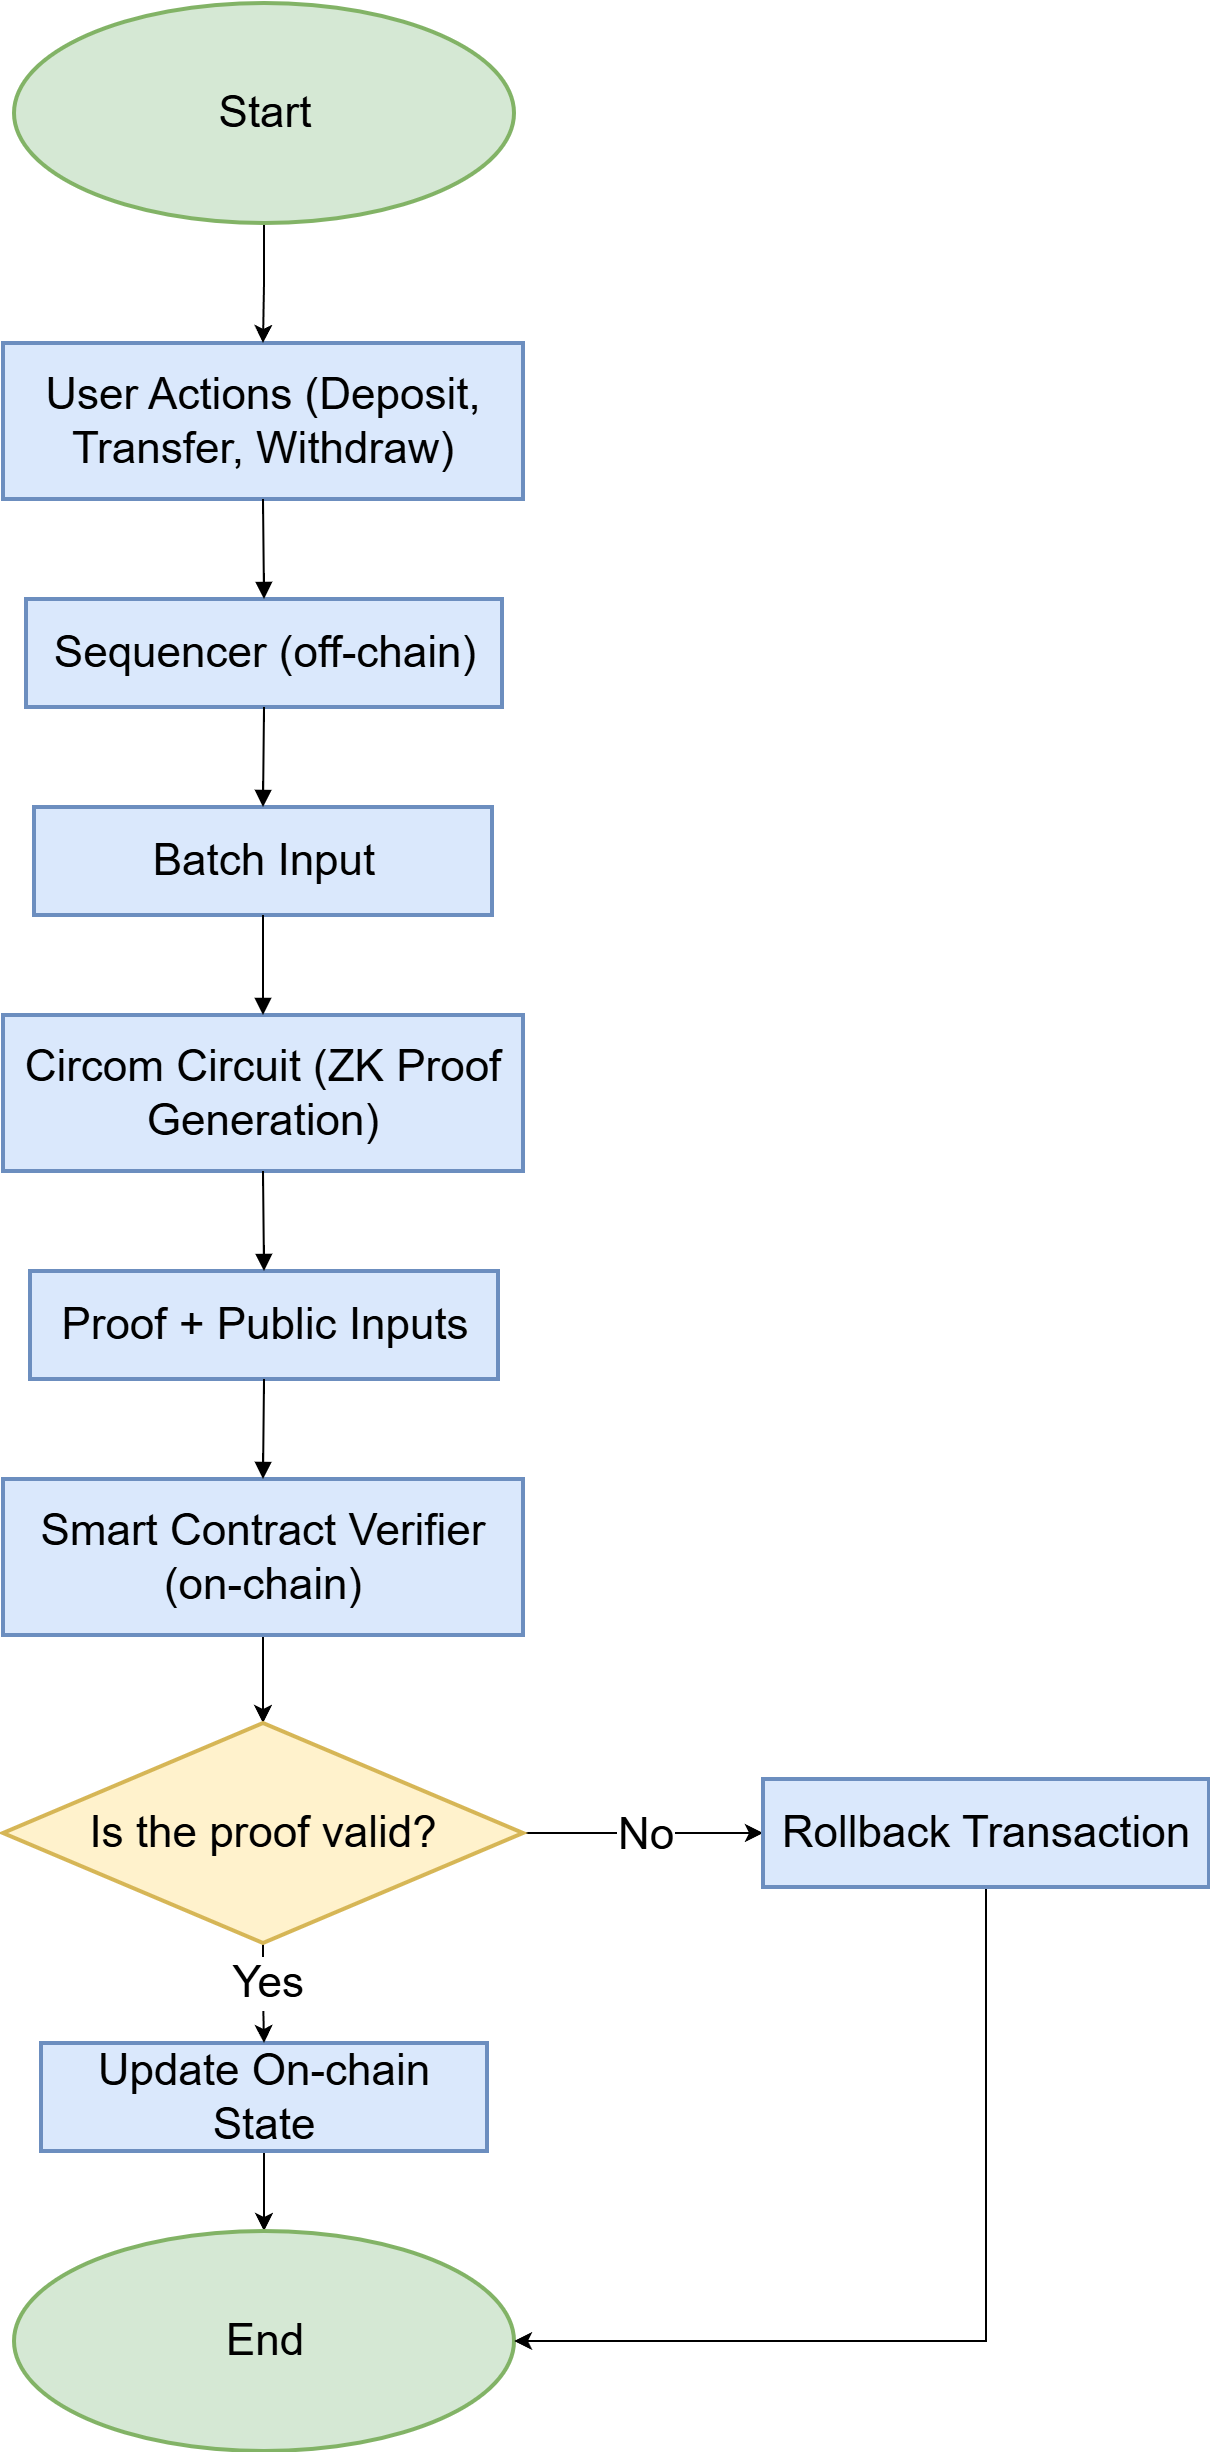
\includegraphics[width = 0.6\textwidth]{imgs/SimpleRollupBaseline.png}
    \caption{Lược đồ mô tả đơn giản hoạt động của các chức năng trong ZK-Rollup mô phỏng}
    \label{fig:chapter4-SimpleRollupBaseline}
\end{figure}

\begin{itemize}
    \item Người dùng khởi tạo một giao dịch (gửi tiền vào layer 2, chuyển tiền giữa các tài khoản, hoặc rút tiền về layer 1). Đối với các giao dịch chuyển và rút tiền, yêu cầu được gửi trực tiếp tới sequencer; đối với gửi tiền, sequencer theo dõi sự kiện từ hợp đồng thông minh layer 1 để ghi nhận. Các giao dịch sau đó được xếp hàng chờ cho đến khi đạt đến ngưỡng lô xác định.
    \item Khi lô giao dịch hoặc yêu cầu rút tiền đã đủ số lượng giao dịch và được chuẩn bị, sequencer tạo ra các đầu vào cho mạch ZK và sử dụng snarkjs để tạo ra ZKP và các tín hiệu công khai.
    \item Bằng chứng và các tín hiệu công khai được gửi tới hợp đồng thông minh tương ứng trên blockchain để xác thực.
    \item Sau khi xác nhận bằng chứng hợp lệ, hợp đồng thông minh cập nhật cây Merkle để cập nhật trạng thái trên chuỗi, trong khi giao dịch cũng được xác nhận ngoài chuỗi bởi sequencer, và được cập nhật trạng thái ngoài chuỗi.
\end{itemize}

% Quy trình chi tiết của hệ thống được minh họa trong Hình 4.2 và có thể được tóm tắt lại trong Hình 4.1 như sau. 
% Trước tiên, người dùng khởi tạo một giao dịch, có thể bao gồm việc gửi tiền vào layer 2, chuyển tiền giữa các tài khoản, hoặc rút tiền về layer 1. Đối với các giao dịch chuyển và rút tiền, yêu cầu được gửi trực tiếp đến sequencer để xử lý. Ngược lại, đối với hoạt động gửi tiền vào layer 2, sequencer sẽ theo dõi các sự kiện phát sinh từ hợp đồng thông minh trên layer 1 nhằm ghi nhận giao dịch tương ứng. Tất cả các giao dịch sau đó được xếp hàng chờ cho đến khi đạt đến ngưỡng xác định để tạo thành một lô giao dịch.

% Khi số lượng giao dịch hoặc yêu cầu rút tiền đã đạt đến ngưỡng cần thiết và sẵn sàng xử lý, sequencer tiến hành tạo các đầu vào phù hợp cho mạch ZK, đồng thời sử dụng công cụ snarkjs để tạo ra bằng chứng không kiến thức (Zero-Knowledge Proof – ZKP) cùng với các tín hiệu công khai tương ứng. Các bằng chứng và tín hiệu công khai này được gửi tới hợp đồng thông minh tương ứng trên blockchain để thực hiện bước xác thực.

% Sau khi hợp đồng thông minh xác nhận bằng chứng là hợp lệ, cây Merkle sẽ được cập nhật để phản ánh trạng thái mới trên chuỗi. Đồng thời, trạng thái ngoài chuỗi của giao dịch cũng được cập nhật bởi sequencer, đảm bảo rằng quá trình xử lý được duy trì nhất quán giữa dữ liệu on-chain và off-chain.


\begin{figure}[h]
    \centering
    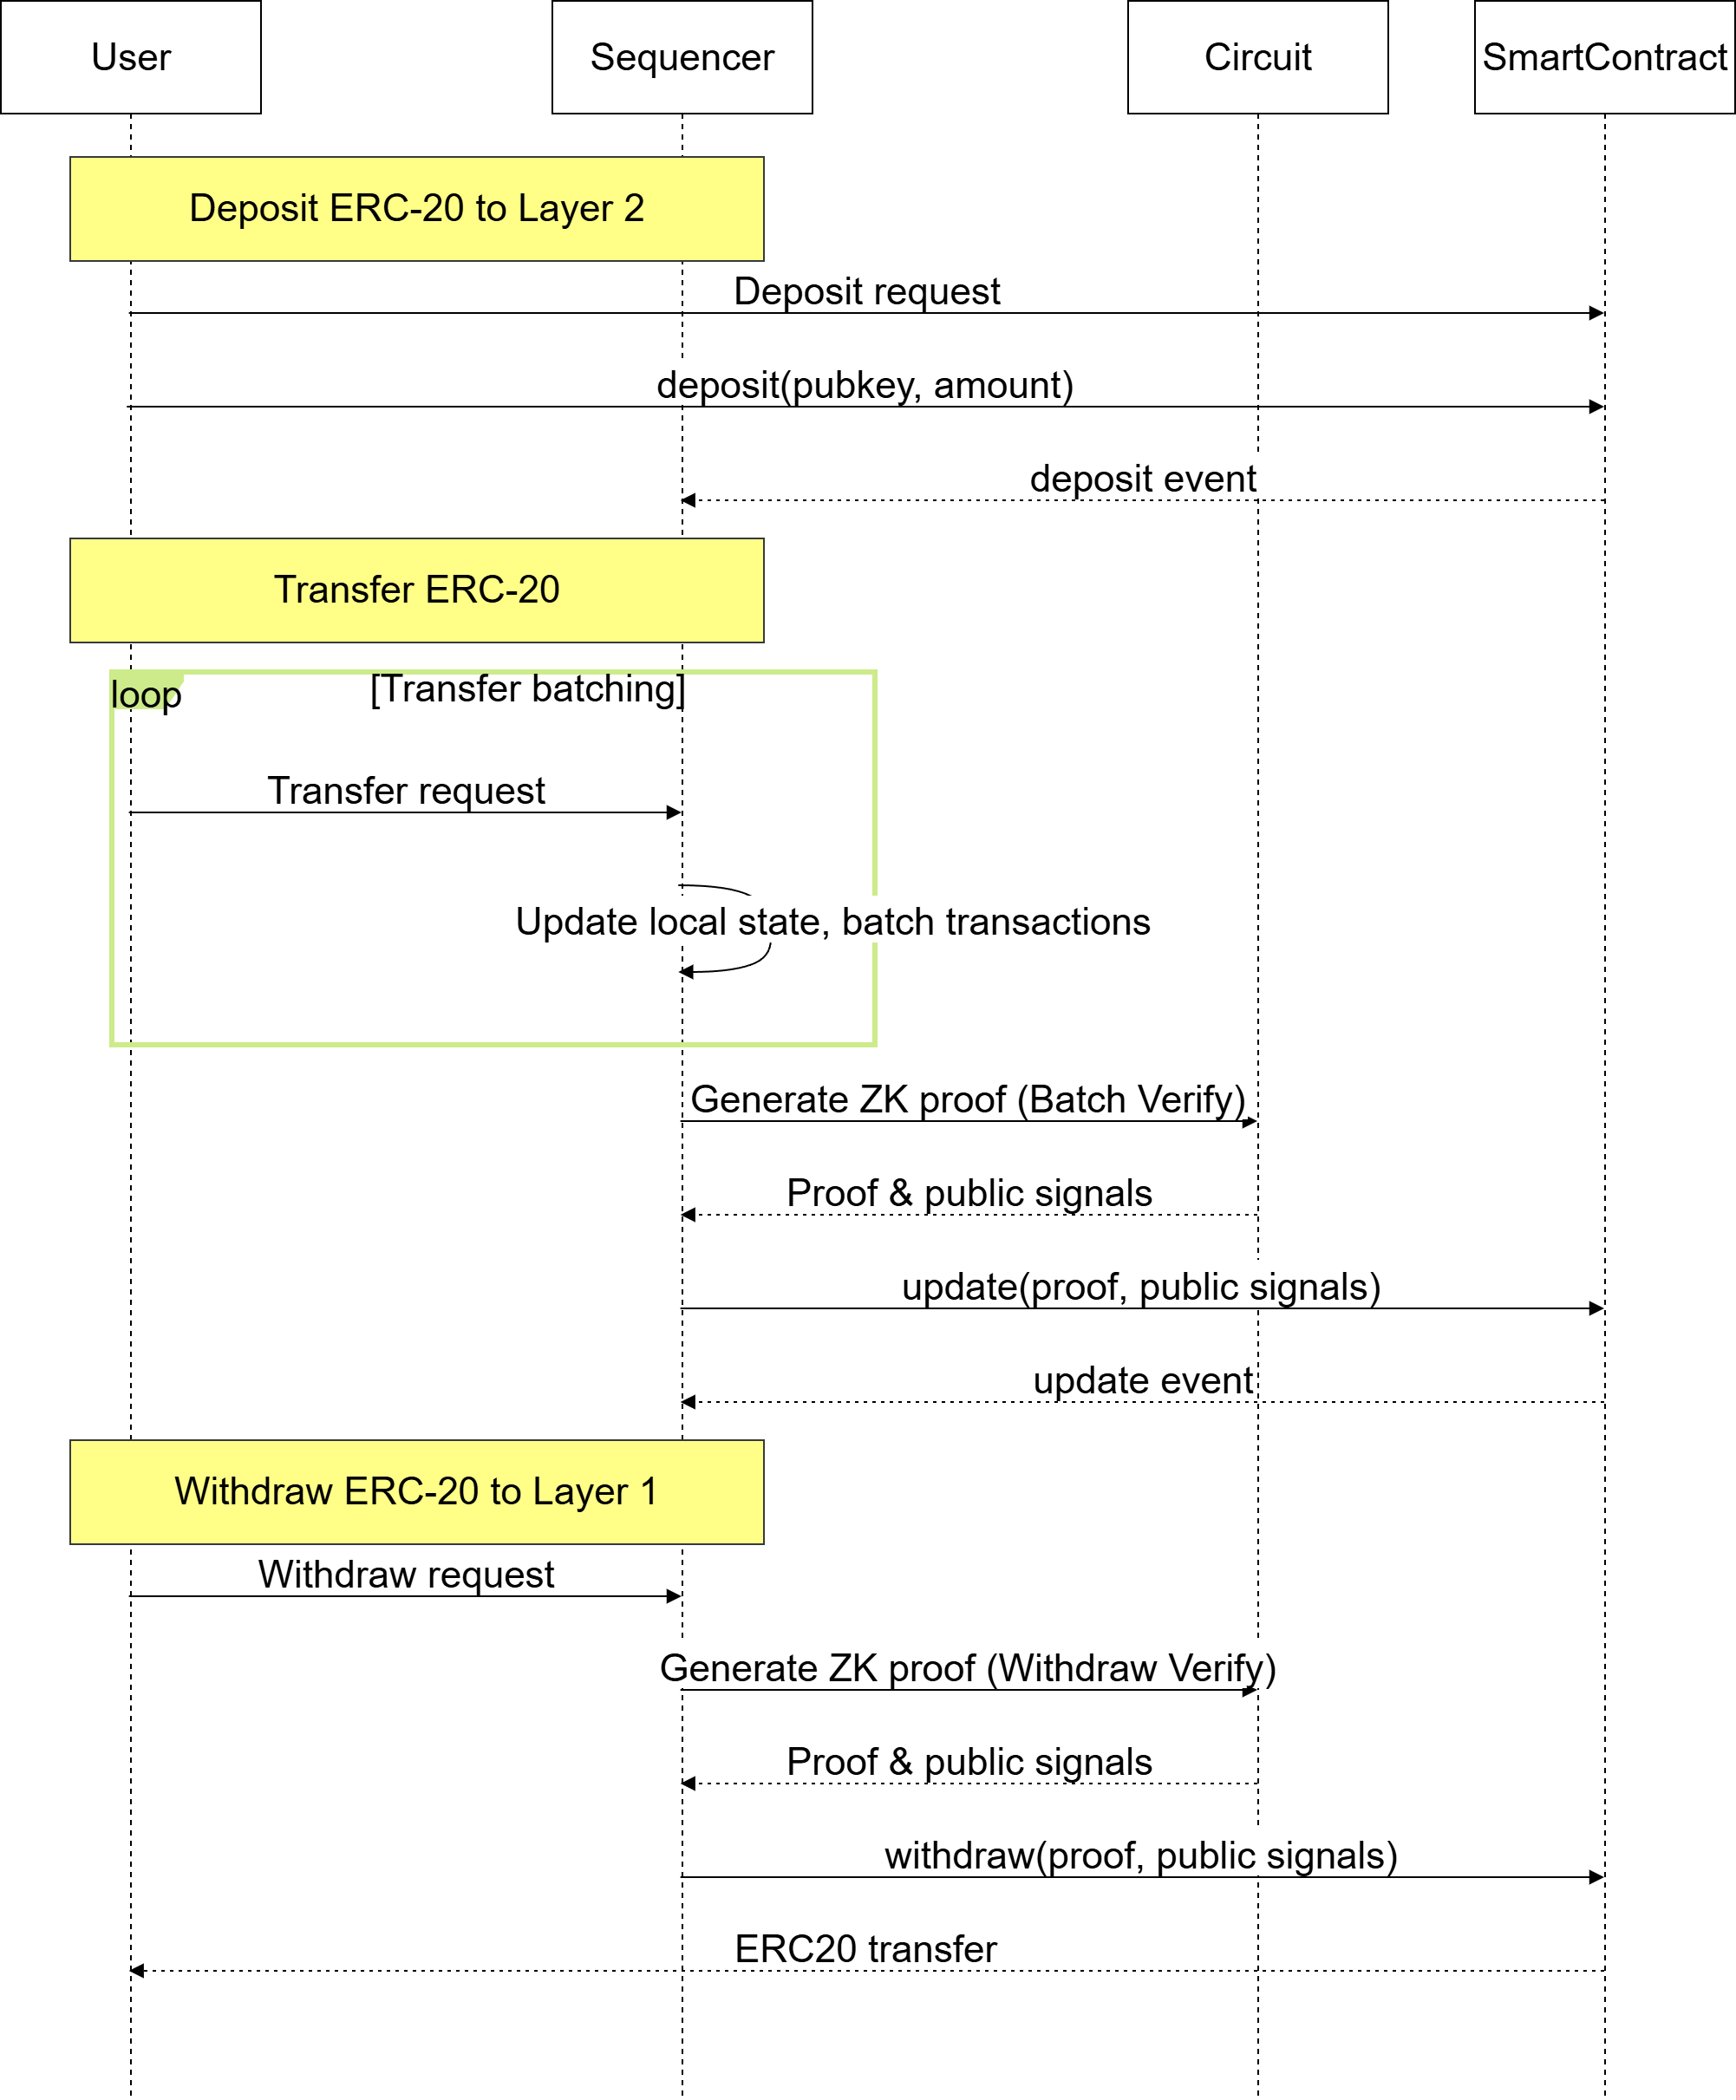
\includegraphics[width = 0.9\textwidth]{imgs/RollupBaseline.png}
    \caption{Lược đồ mô tả chi tiết hoạt động của các chức năng trong ZK-Rollup mô phỏng}
    \label{fig:chapter4-RollupBaseline}
\end{figure}
\clearpage
\section{Phương pháp đề xuất: ZK Circuit Lifecycle Strategy (ZCLS)}

Các kết quả thực nghiệm nhấn mạnh rằng thời gian biên dịch là một rào cản phát triển đáng kể cho các triển khai ZK-Rollup quy mô lớn. Mặc dù cần thiết phải sử dụng --O2 để đảm bảo sinh chứng minh hiệu quả, sự đánh đổi với thời gian biên dịch tăng lên có thể làm gián đoạn quy trình làm việc khi phát triển ứng dụng. Do đó, việc lựa chọn cờ tối ưu hóa ràng buộc của trình biên dịch mạch một cách phù hợp có vai trò quan trọng và cần được cân nhắc kĩ lưỡng. Dựa trên các phân tích thực nghiệm về tác động của các mức tối ưu hoá ràng buộc của Circom, nghiên cứu này đề xuất một phương pháp luận có cấu trúc, được gọi là ZCLS. Phương pháp ZCLS cung cấp một khung hướng dẫn cho các nhà phát triển trong việc đưa ra quyết định sáng suốt về tối ưu hóa mạch ZKP xuyên suốt các giai đoạn khác nhau của quá trình phát triển và triển khai.

\subsection{Giới thiệu về ZCLS}
ZCLS là một phương pháp tiếp cận nhằm quản lý và tối ưu hóa quá trình biên dịch mạch ZKP, từ giai đoạn thiết kế ban đầu cho đến triển khai sản phẩm. Mục tiêu của ZCLS là cân bằng giữa tốc độ phát triển (thời gian biên dịch) và hiệu suất thực thi (thời gian tạo bằng chứng), dựa trên các yêu cầu cụ thể của từng giai đoạn. ZCLS hoạt động với nhận thức rằng không có một cờ tối ưu hóa nào là ``tốt nhất'' cho mọi tình huống; thay vào đó, lựa chọn tối ưu phụ thuộc vào các yếu tố như tần suất cập nhật mạch, khối lượng bằng chứng cần tạo, và giai đoạn hiện tại của dự án.

\subsection{Các yếu tố quyết định trong ZCLS}
ZCLS xem xét ba yếu tố chính để đưa ra khuyến nghị về cờ tối ưu hóa:
\begin{enumerate}
    \item \textbf{Giai đoạn Phát triển (Development Stage)}

    Đây là yếu tố đầu tiên và quan trọng nhất, xác định ưu tiên chính của quá trình tối ưu hóa:
    \begin{itemize}
        \item \textbf{Phát triển và Thử nghiệm (Development and Testing):} Trong giai đoạn này, mạch ZKP thường xuyên được thay đổi, bổ sung tính năng, và gỡ lỗi. Ưu tiên hàng đầu là tốc độ biên dịch nhanh để rút ngắn chu kỳ phản hồi và tăng hiệu quả làm việc của nhà phát triển. Hiệu suất tạo bằng chứng vẫn quan trọng cho việc kiểm thử, nhưng không phải là yếu tố quyết định tuyệt đối.
        \item \textbf{Triển khai Thực tế (Production Deployment): }Khi mạch đã ổn định và sẵn sàng cho môi trường sản phẩm, ưu tiên chuyển sang hiệu suất tạo bằng chứng tối đa và ổn định. Tần suất cập nhật mạch giảm đáng kể, do đó thời gian biên dịch dài hơn có thể được chấp nhận. 
        \item \textbf{Trường Hợp Đặc Biệt (Gỡ Lỗi - Debugging): }Trong các tình huống cần gỡ lỗi sâu hoặc kiểm tra nhanh các phần nhỏ của mạch, tốc độ biên dịch là yếu tố quan trọng nhất, thậm chí hy sinh hiệu suất tạo bằng chứng.
    \end{itemize}
    
    \item \textbf{Tần suất cập nhật mạch (Circuit Update Frequency)}

    ``Tần suất cập nhật mạch'' đề cập đến số lần cập nhật mạch trong quá trình phát triển, tức là số lần nhà phát triển thay đổi mã nguồn của mạch và cần biên dịch lại. Yếu tố này ảnh hưởng trực tiếp đến thời gian chờ đợi của nhà phát triển. Tần suất cập nhật mạch càng cao, yêu cầu về thời gian biên dịch càng nhanh để không làm gián đoạn quy trình làm việc. Các ngưỡng định lượng được gợi ý giúp nhà phát triển tham chiếu và sử dụng khung hướng dẫn một cách dễ dàng hơn.

    % Dựa trên dữ liệu benchmark của chúng tôi (đặc biệt tại lô giao dịch 64, đại diện cho kịch bản tải cao nhất trong thử nghiệm hiện tại), chúng tôi định lượng tác động của tần suất cập nhật mạch đến yêu cầu về thời gian biên dịch như sau:

    \begin{itemize}
        \item \textbf{Cao (High Frequency):} Tần suất này thường xuất hiện ở giai đoạn phát triển và thử nghiệm lặp lại, nơi các thay đổi mạch diễn ra thường xuyên (\textit{ví dụ:} nhiều lần trong một giờ hoặc một ngày). Trong giai đoạn này, thời gian biên dịch của mỗi lần thay đổi là yếu tố quan trọng. Yều cầu về thời gian biên dịch của giai đoạn này là \textit{nhanh}. \textbf{Ngưỡng định lượng đề xuất:} Từ 10 - 50 lần/ngày.
        % Dựa trên dữ liệu của chúng tôi, thời gian biên dịch của --O0 (\textasciitilde 46 giây) và --O1 (\textasciitilde 64 giây) tại kích thước lô 64 là chấp nhận được cho các vòng lặp phát triển nhanh. Thời gian biên dịch của --O2 (\textasciitilde 122 giây) có thể gây ra sự chậm trễ đáng kể.
        
        % \textbf{Ngưỡng định lượng:} Yêu cầu thời gian biên dịch nhanh -- Chọn dưới 65 giây cho kích thước lô 64 (sử dụng --O0 hoặc --O1). 

        \item \textbf{Thấp (Low Frequency):} Áp dụng cho các mạch đã ổn định, hiếm khi được cập nhật, chỉ khi có các bản nâng cấp lớn, vá lỗi bảo mật nghiêm trọng hoặc thay đổi giao thức cốt lõi. Trong trường hợp này, yêu cầu về thời gian biên dịch mạch là \textit{không quan trọng}. \textbf{Ngưỡng định lượng đề xuất:} dưới 1 lần/tuần (\textit{ví dụ:} 1 lần/tháng, 1 lần/quý, hoặc ít hơn).
        % Trong trường hợp này, thời gian biên dịch dài hơn của --O2 là chấp nhận được vì nó không ảnh hưởng đáng kể đến năng suất tổng thể.

        % \textbf{Ngưỡng định lượng:} Yêu cầu thời gian biên dịch chấp nhận được -- trên 65 giây cho Batch Size 64 (sử dụng --O2).

        \item \textbf{Rất Cao -- Dùng khi gỡ lỗi (Very High Frequency for Debugging):} Khi tốc độ biên dịch là ưu tiên tuyệt đối để gỡ lỗi nhanh, ngay cả khi hiệu suất tạo bằng chứng không tối ưu. Trong trường hợp này, yêu cầu về thời gian biên dịch sẽ là \textit{rất nhanh}. \textbf{Ngưỡng định lượng đề xuất:} Trên 50 lần/ngày (hoặc nhiều lần mỗi giờ).
        % Điều này chỉ có thể đạt được với --O0.

        % \textbf{Ngưỡng định lượng:} Yêu cầu thời gian biên dịch tối thiểu -- dưới 50 giây cho kích thước lô 64 (sử dụng --O0).
    \end{itemize}
    
    \item \textbf{Khối lượng tạo bằng chứng (Proof Generation Volume)}

    ``Khối lượng tạo bằng chứng'' đề cập đến số lượng bằng chứng dự kiến sẽ tạo ra để kiểm tra hệ thống, tức là quy mô của các bài kiểm tra hoặc số lượng giao dịch cần được xử lý trong một lô để xác minh. Yếu tố này ảnh hưởng trực tiếp đến thời gian tạo bằng chứng và khả năng mở rộng của hệ thống.

    % Dựa trên dữ liệu benchmark của chúng tôi (tại kích thước lô 64), chúng tôi định lượng tác động của khối lượng tạo bằng chứng đến yêu cầu về thời gian tạo bằng chứng như sau:

    \begin{itemize}
    
    \item \textbf{Cao (High Volume):} Khối lượng này sẽ xảy ra với các trường hợp cần tạo bằng chứng cho các lô giao dịch lớn hoặc khi cần tạo bằng chứng liên tục để kiểm thử thông lượng của hệ thống. Đây là nơi tối ưu hóa thời gian tạo bằng chứng (như --O2) trở nên cực kỳ quan trọng. Yêu cầu về thời gian tạo bằng chứng ở trường hợp này sẽ là \textit{nhanh}. \textbf{Ngưỡng định lượng đề xuất:} 
    Trên 100 bằng chứng/ngày.
    
    % Dựa trên dữ liệu của chúng tôi, thời gian tạo bằng chứng của --O2 (\textasciitilde 29 giây) và --O1 (\textasciitilde 37 giây) tại kích thước lô 64 là phù hợp cho các kịch bản này.

    % \textbf{Ngưỡng định lượng:} Yêu cầu thời gian tạo bằng chứng nhanh -- dưới 40 giây cho kích thước lô 64 (sử dụng --O1 hoặc --O2).

    \item \textbf{Thấp (Low Volume):} Ám chỉ các trường hợp cần tạo bằng chứng không thường xuyên hoặc cho các lô giao dịch nhỏ trong quá trình kiểm thử. Yêu cầu về thời gian tạo bằng chứng của trường hợp này sẽ là \textit{trung bình}. \textbf{Ngưỡng định lượng đề xuất:} Từ 50 - 100 bằng chứng/ngày.
    
    % Thời gian tạo bằng chứng dài hơn của --O0 (\textasciitilde75 giây) là chấp nhận được.

    % \textbf{Ngưỡng định lượng:} Yêu cầu thời gian tạo bằng chứng chấp nhận được -- trên 40 giây cho kích thước lô 64 (sử dụng --O0).

    \item \textbf{Rất Thấp (Very Low Volume for Debugging):} Khi thời gian tạo bằng chứng không phải là mối quan tâm, ưu tiên tuyệt đối sẽ dành cho tốc độ biên dịch, ngay cả khi hiệu suất tạo bằng chứng không tối ưu. Điều này tương ứng với hiệu suất của --O0 với yêu cầu về thời gian biên dịch là \textit{rất nhanh}. \textbf{Ngưỡng định lượng đề xuất:} Dưới 1 bằng chứng/giờ (\textit{ví dụ:} 1 bằng chứng/ngày hoặc ít hơn).

    % \textbf{Ngưỡng định lượng:} Yêu cầu thời gian tạo bằng chứng không quan trọng -- trên 70 giây cho kích thước lô 64 (sử dụng --O0).
    \end{itemize}
\end{enumerate}

\subsection{Bảng và khung khuyến nghị ZCLS}
Dựa trên các yếu tố định tính và yêu cầu hiệu suất tương ứng, bảng khuyến nghị ZCLS được trình bày trong bảng \ref{tab:optimization_flag_selection} và hình \ref{fig:chapter4-FrameworkCircom}.

\begin{table}[h]
    \centering
    \caption{Các mức tối ưu hóa trình biên dịch Circom được khuyến nghị dựa trên giai đoạn phát triển, tần suất cập nhật mạch và khối lượng bằng chứng được tạo.}
    \resizebox{\textwidth}{!}{%
    \begin{tabular}{|l|l|l|l|}
        \hline
        \textbf{Giai Đoạn Phát Triển} & \textbf{Tần Suất Cập Nhật Mạch} & \textbf{Khối Lượng Tạo Bằng Chứng} & \textbf{Cờ Được Khuyến Nghị} \\
        \hline
        Trường Hợp Đặc Biệt (Gỡ Lỗi) & Rất Cao (Thường Xuyên) & Rất Thấp & --O0 \\
        Phát Triển, Thử Nghiệm & Cao & Thấp & --O1 \\
        Phát Triển, Thử Nghiệm & Cao & Cao & --O1 \\
        Triển Khai Thực Tế & Thấp & Cao & --O2 \\
        Triển Khai Thực Tế & Thấp & Thấp & --O2 \\
        \hline
    \end{tabular}
    }
    \label{tab:optimization_flag_selection}
\end{table}

% ver 1
%\clearpage
% \begin{figure}[h] % 'h' để đặt ảnh gần vị trí lệnh
%     \centering % Căn giữa ảnh
%     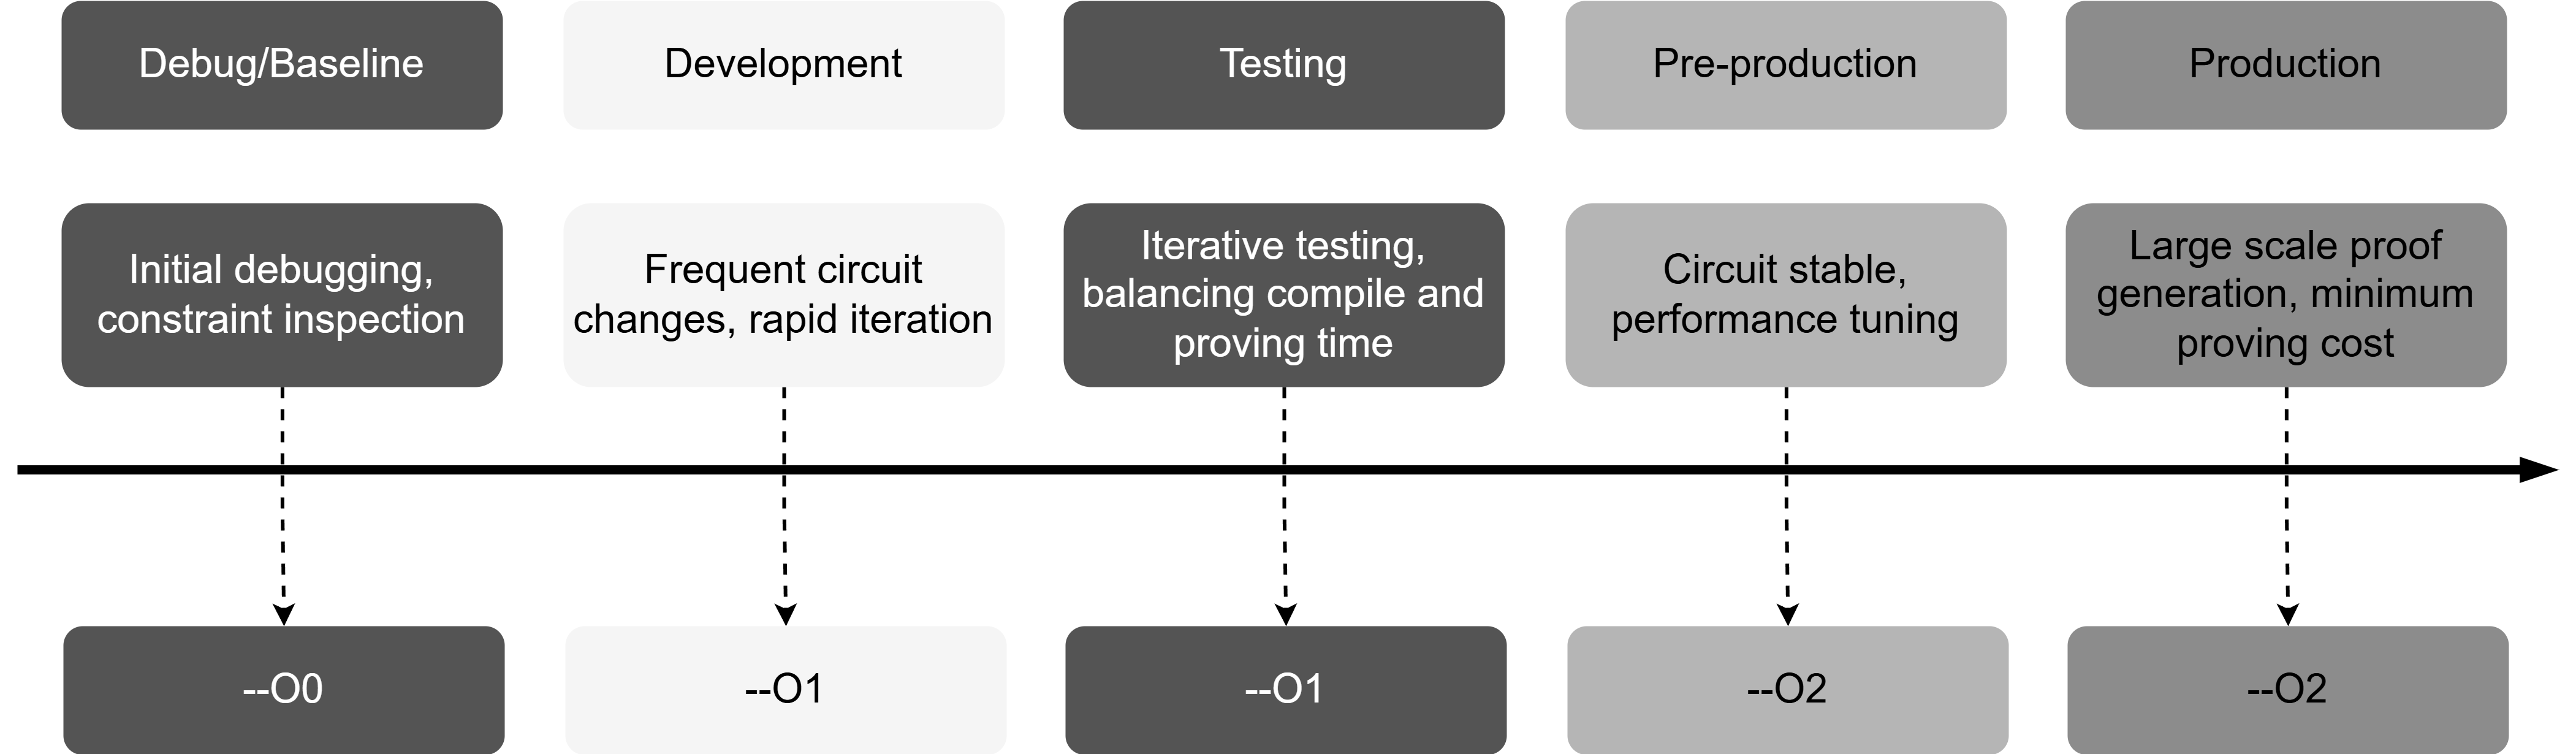
\includegraphics[width=\textwidth]{imgs/framework.png}
%     \caption{Khung chọn cờ tối ưu hóa trình biên dịch Circom dựa trên giai đoạn phát triển, tần suất cập nhật mạch và khối lượng tạo bằng chứng}
%     \label{fig:chapter4-framework}
% \end{figure}

% ver 2
% \begin{figure}[h] % 'h' để đặt ảnh gần vị trí lệnh
%     \centering % Căn giữa ảnh
%     \rotatebox{90}{
%     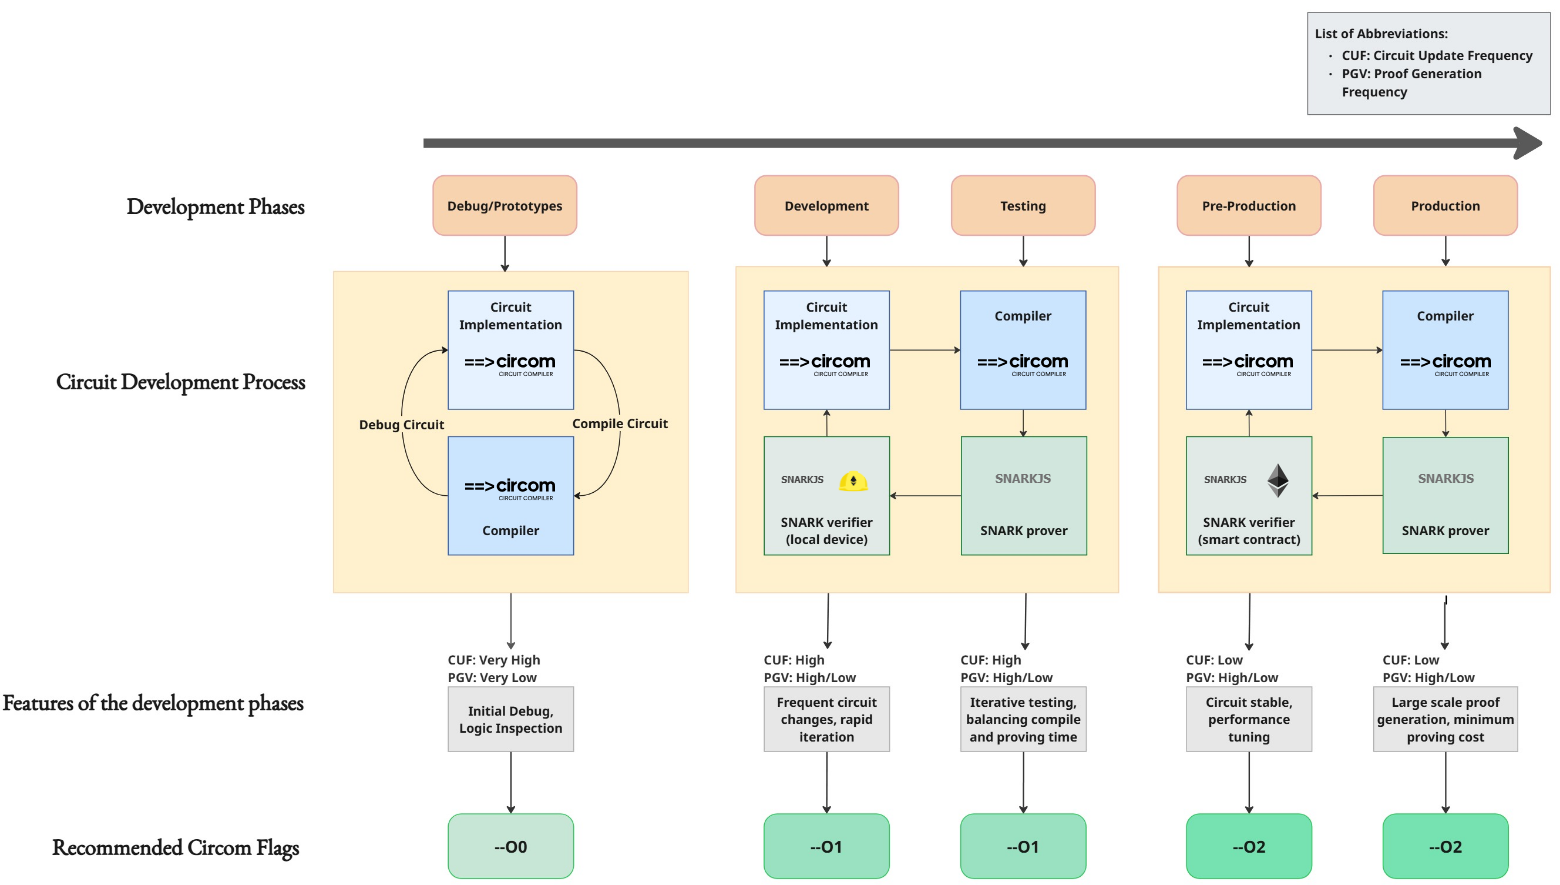
\includegraphics[height=0.7\textwidth]{imgs/FrameworkCircom.drawio.png}}
%     \caption{Khung chọn cờ tối ưu hóa trình biên dịch Circom dựa trên giai đoạn phát triển, tần suất cập nhật mạch và khối lượng tạo bằng chứng}
%     \label{fig:chapter4-FrameworkCircom1}
% \end{figure}

% ver 3
% \begin{figure}[h] % 'h' để đặt ảnh gần vị trí lệnh
%     \centering % Căn giữa ảnh
%     \rotatebox{90}{
%     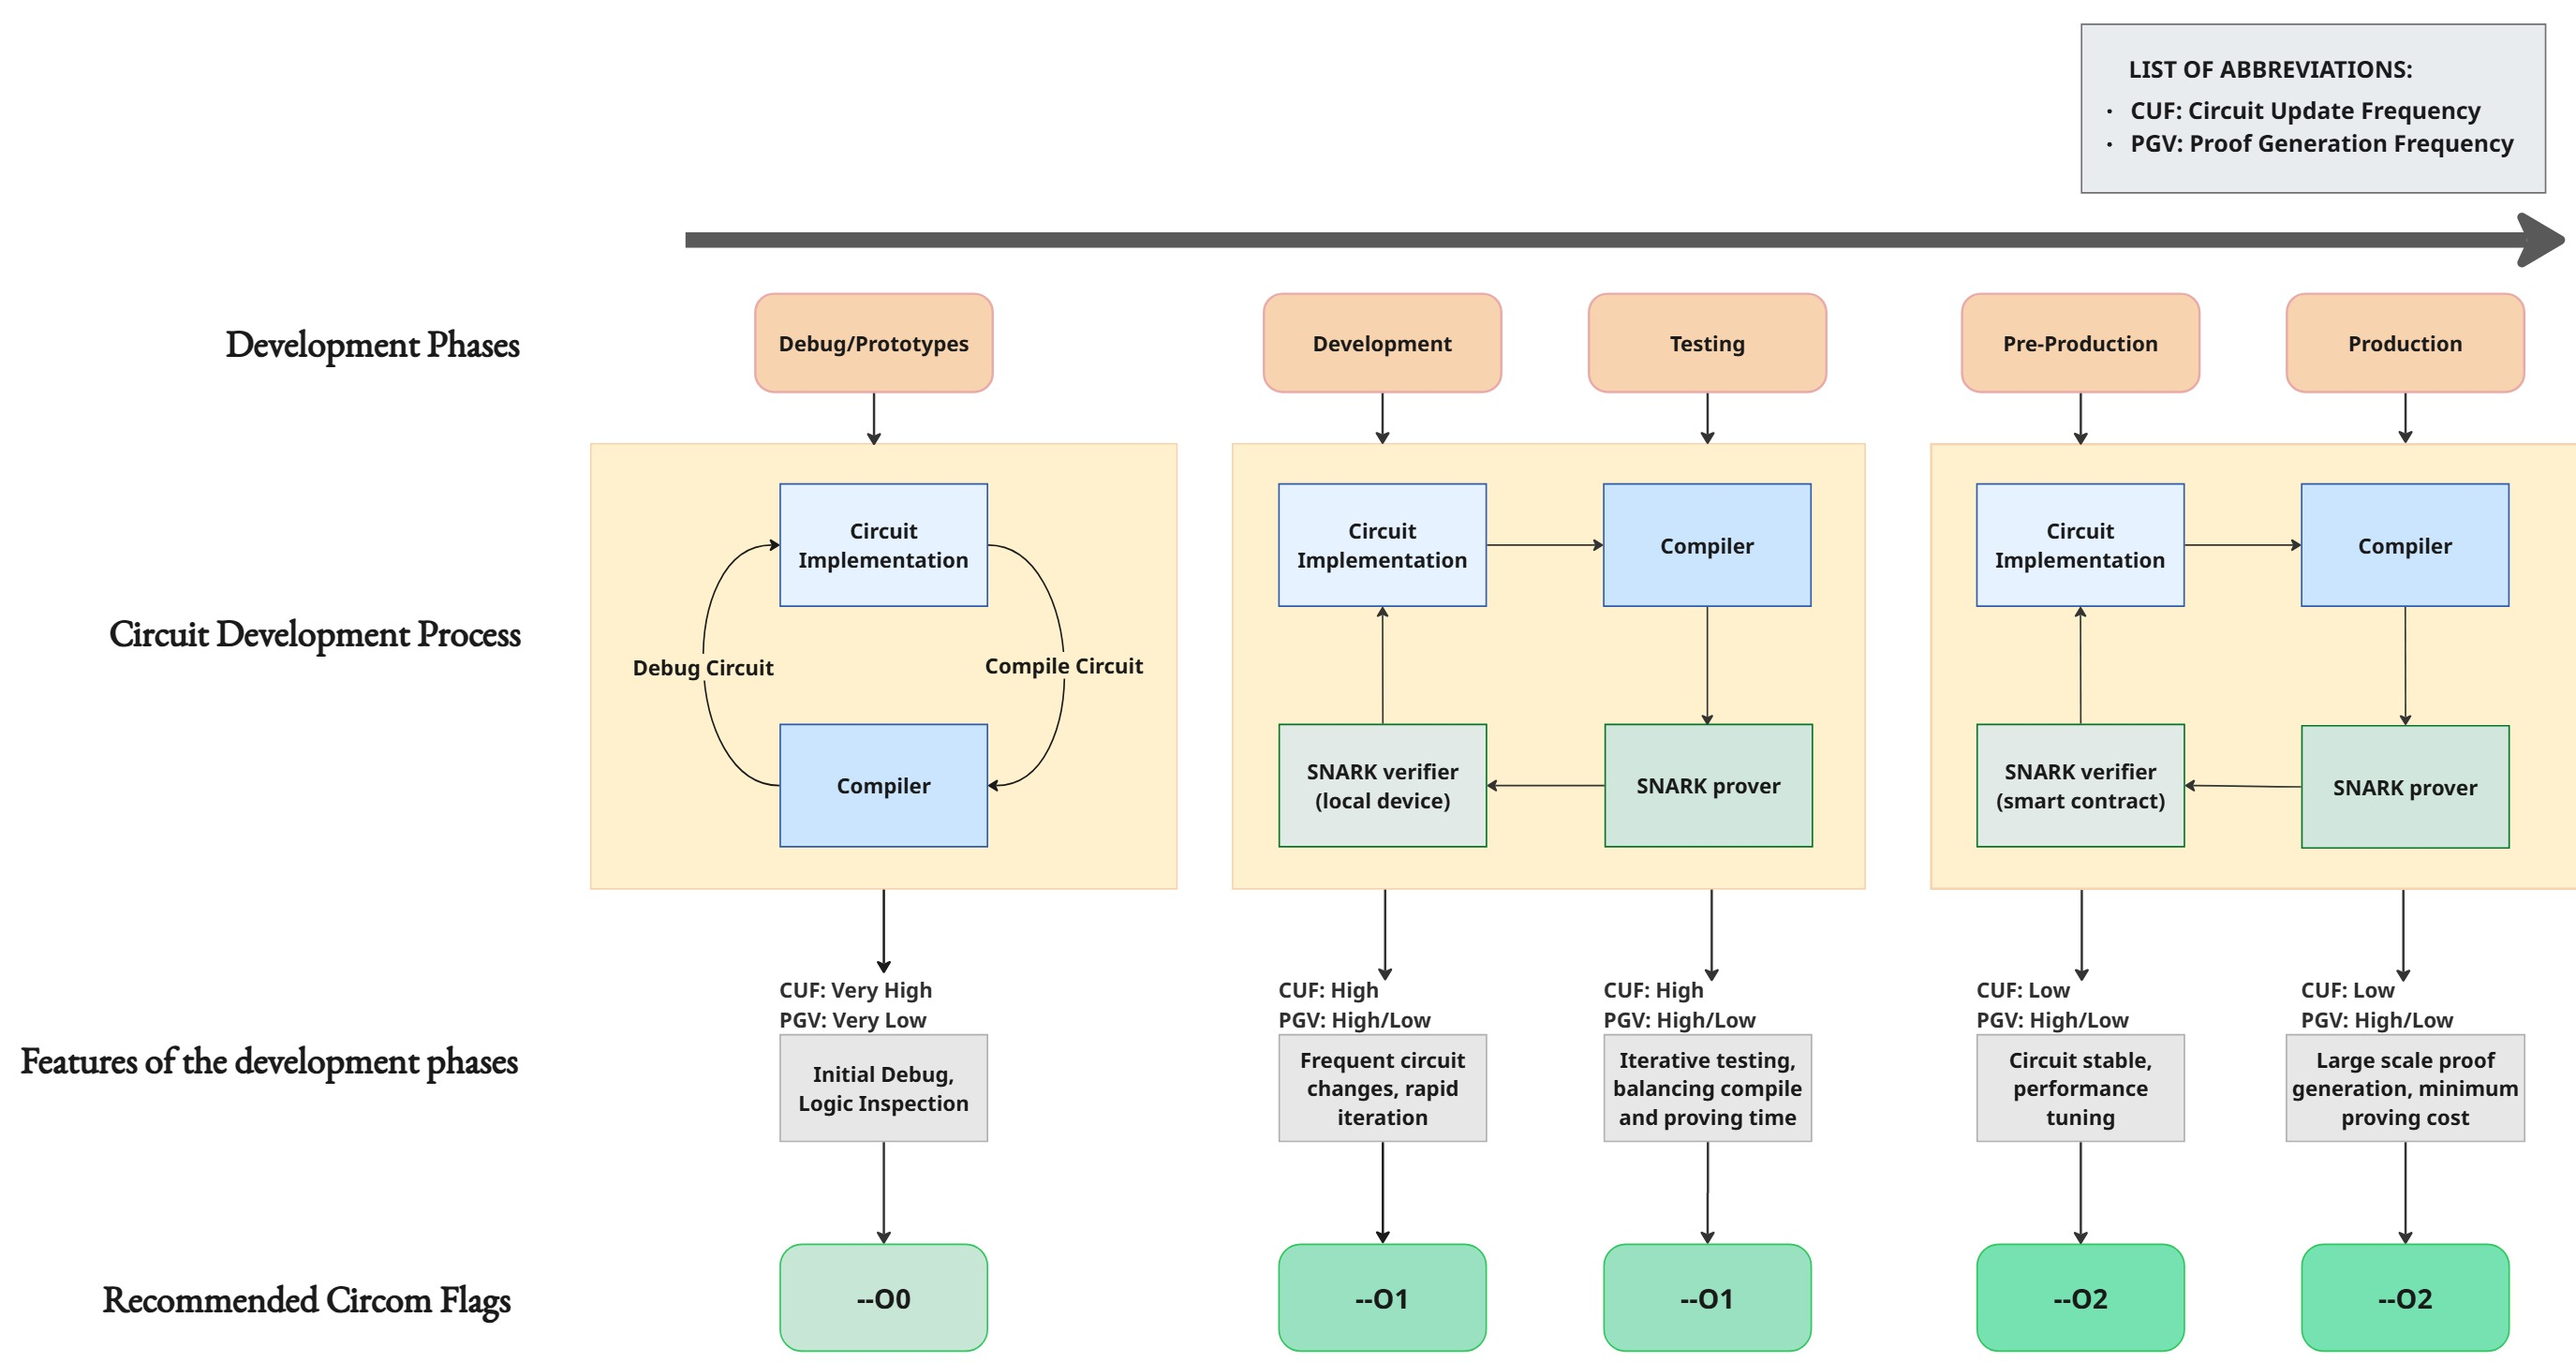
\includegraphics[height=0.7\textwidth]{imgs/FrameworkCircom.jpg}}
%     \caption{Khung chọn cờ tối ưu hóa trình biên dịch Circom dựa trên giai đoạn phát triển, tần suất cập nhật mạch và khối lượng tạo bằng chứng}
%     \label{fig:chapter4-FrameworkCircom}
% \end{figure}

% \begin{figure}[h] % 'h' để đặt ảnh gần vị trí lệnh
%     \centering % Căn giữa ảnh
%     \rotatebox{90}{
%     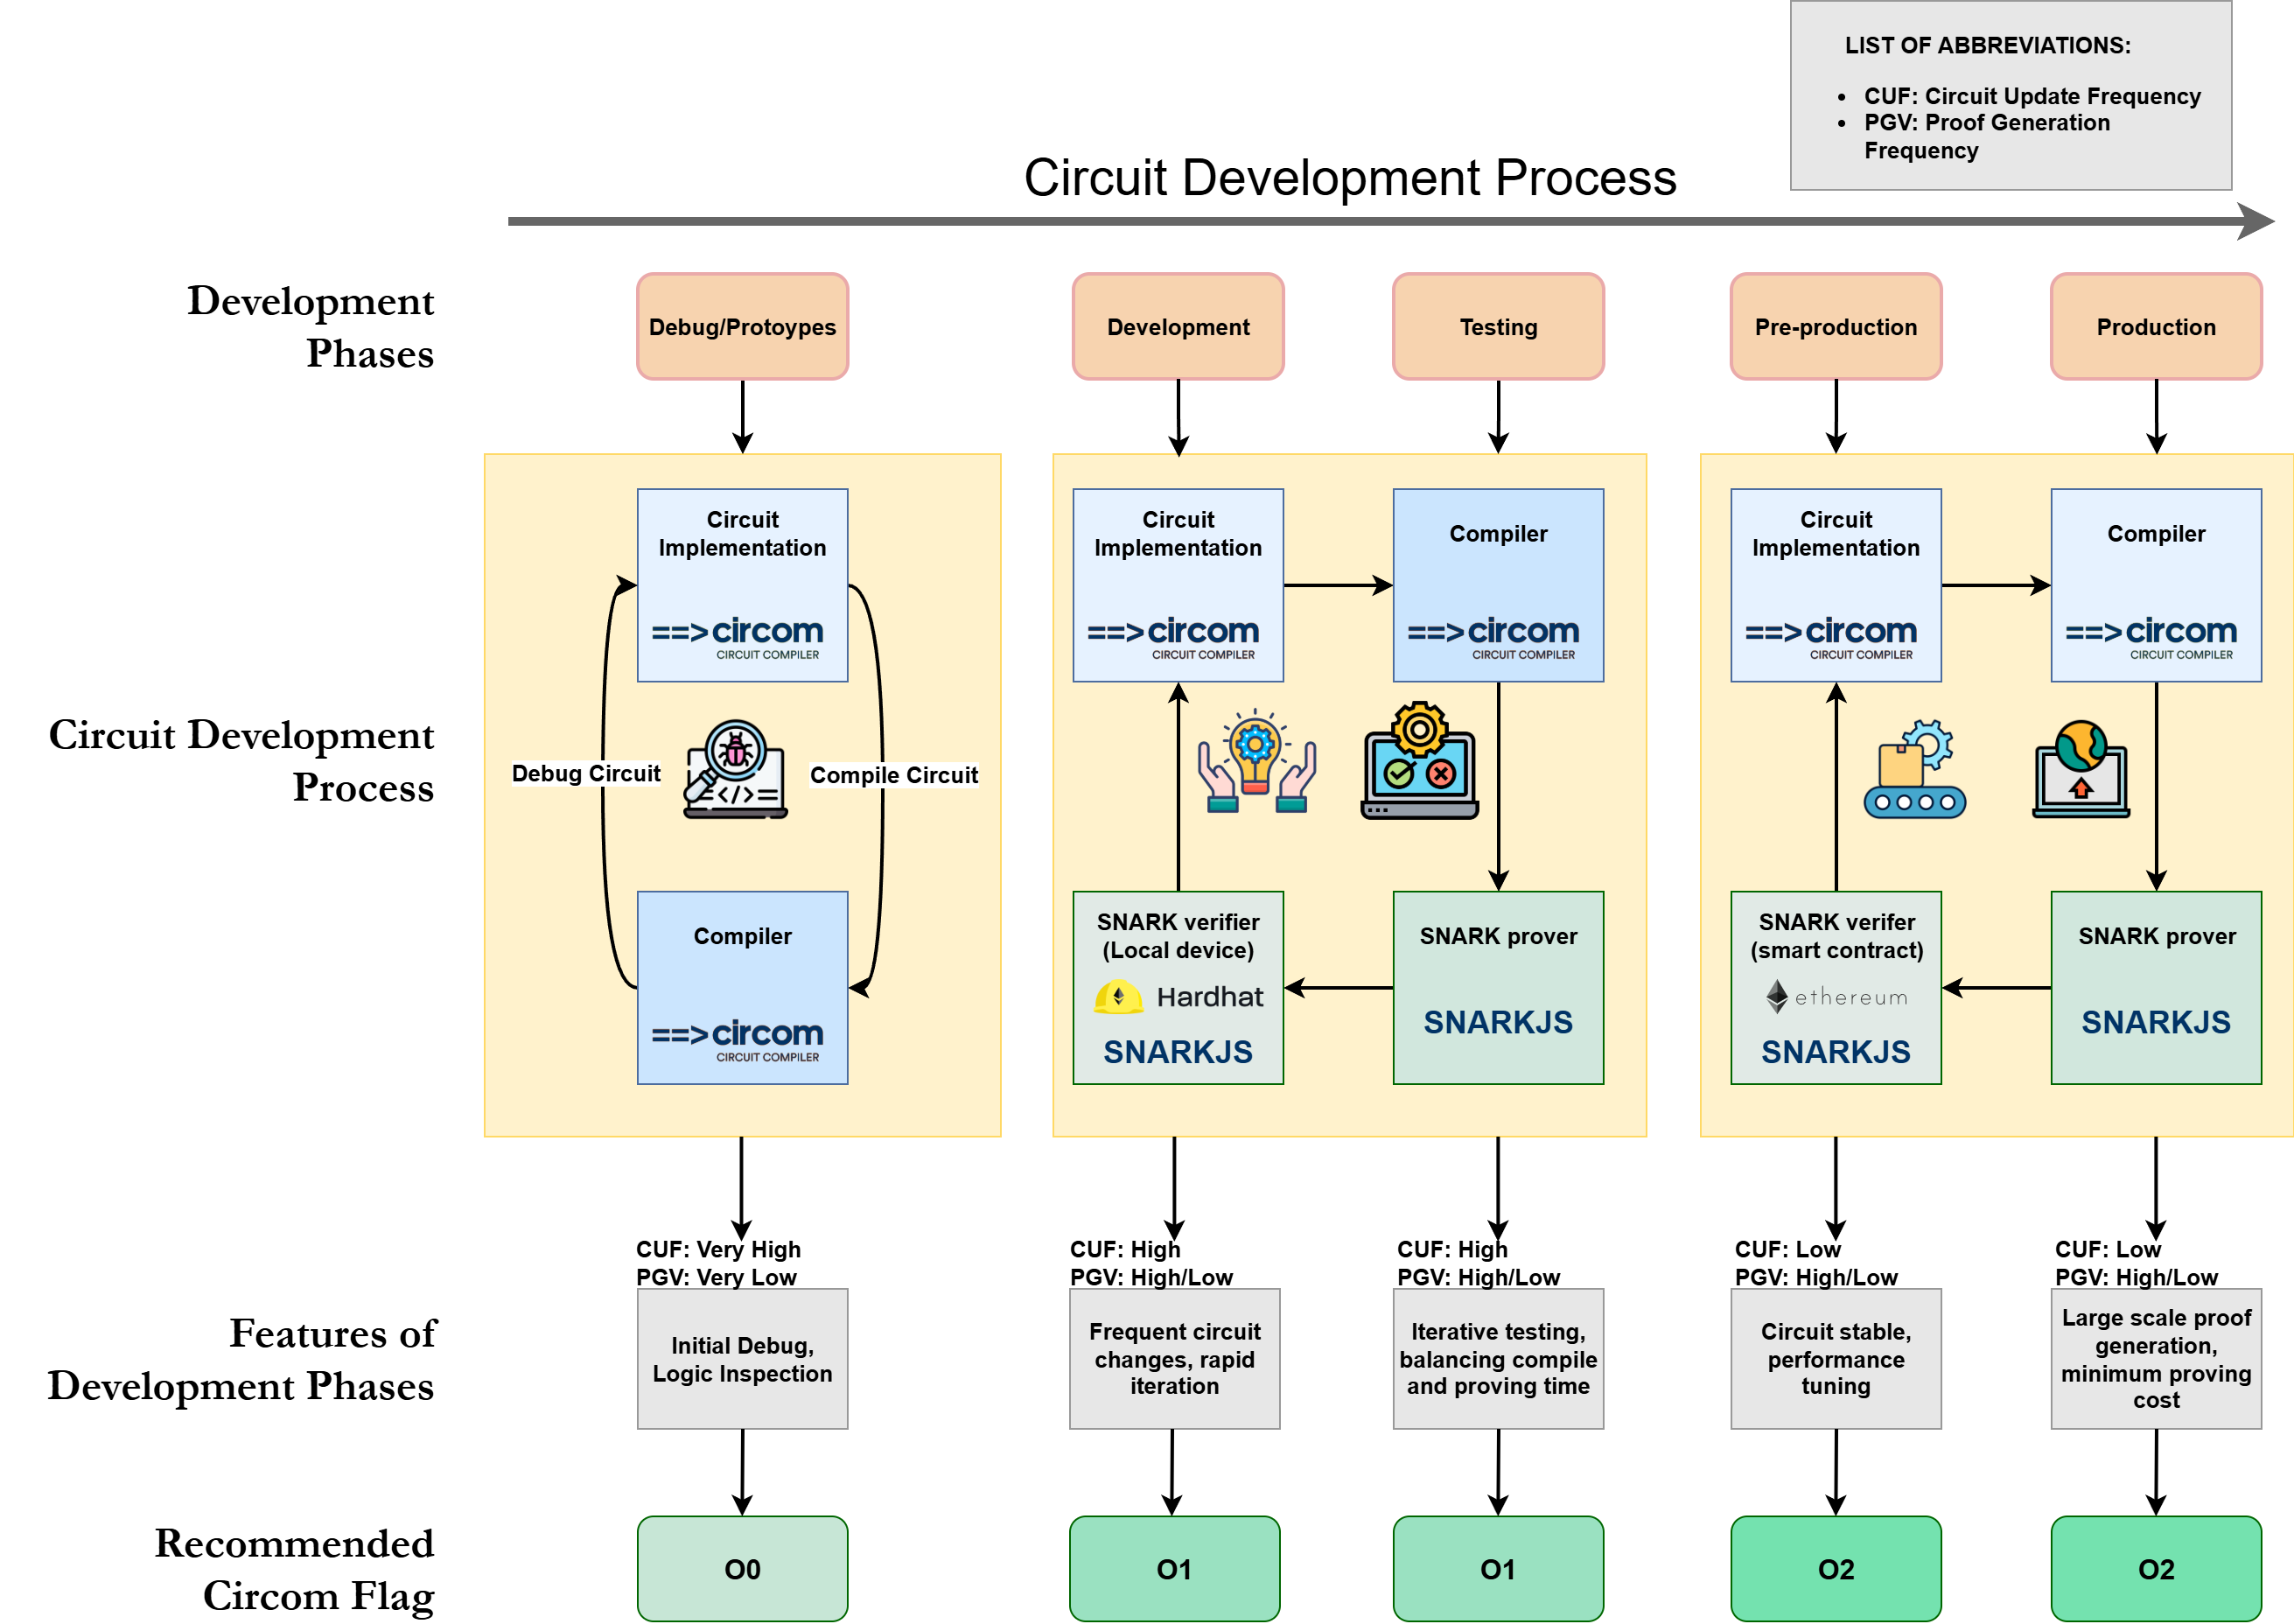
\includegraphics[height=0.9\textwidth]{imgs/FlagSelection.png}}
%     \caption{Khung chọn cờ tối ưu hóa trình biên dịch Circom dựa trên giai đoạn phát triển, tần suất cập nhật mạch và khối lượng tạo bằng chứng}
%     \label{fig:chapter4-FrameworkCircom}
% \end{figure}

Các khuyến nghị trong khung và bảng trên được xây dựng dựa trên sự đánh đổi giữa thời gian biên dịch và thời gian tạo bằng chứng, được định lượng từ dữ liệu thực nghiệm của nghiên cứu (đặc biệt tại kích thước lô 64, đại diện cho kịch bản lô cao nhất trong thử nghiệm hiện tại). Dưới đây là phần giải thích cho từng trường hợp cụ thể:

\begin{enumerate}
    \item \textbf{Phát Triển, Thử Nghiệm (Development, Testing):}
    \begin{itemize}
        \item \textbf{Tần Suất Cập Nhật Mạch: Cao} -- \textbf{Yêu cầu thời gian biên dịch nhanh}:
        \begin{itemize}
            \item \textbf{Khối Lượng Tạo Bằng Chứng: Thấp} -- \textbf{Yêu cầu thời gian tạo bằng chứng trung bình}: Trong kịch bản này, ưu tiên hàng đầu là tốc độ biên dịch để nhà phát triển có thể lặp lại quá trình biên dịch nhanh chóng. --O1 được khuyến nghị vì nó cung cấp thời gian biên dịch nhanh (\textasciitilde 64s) và thời gian tạo bằng chứng chấp nhận được (\textasciitilde 37s), là sự cân bằng tốt nhất. --O0 biên dịch nhanh hơn nhưng thời gian tạo bằng chứng quá chậm (\textasciitilde 75s) có thể làm chậm quá trình kiểm thử, trong khi --O2 có thời gian biên dịch quá dài (\textasciitilde 122s).
            \item \textbf{Khối Lượng Tạo Bằng Chứng: Cao} -- \textbf{Yêu cầu thời gian tạo bằng chứng nhanh}: Ngay cả khi cần tạo bằng chứng nhanh cho các bài kiểm thử tải cao, --O1 vẫn là lựa chọn cân bằng. Nó cung cấp thời gian biên dịch nhanh (\textasciitilde 64s) và thời gian tạo bằng chứng đủ nhanh (\textasciitilde 36s) để kiểm thử các kịch bản tải cao mà không phải chịu chi phí biên dịch quá lớn của --O2. Điều này cho phép nhà phát triển nhanh chóng kiểm tra hiệu suất mạch mà không bị cản trở bởi thời gian biên dịch kéo dài.
        \end{itemize}
    \end{itemize}

    \item \textbf{Triển Khai Thực Tế (Production Deployment):}
    \begin{itemize}
        \item \textbf{Tần Suất Cập Nhật Mạch: Thấp} -- \textbf{Yêu cầu thời gian biên dịch trung bình}: Khi mạch đã ổn định và sẵn sàng cho môi trường sản phẩm, tần suất cập nhật mạch giảm đáng kể, do đó thời gian biên dịch dài hơn của --O2 (\textasciitilde 122s) là chấp nhận được.
        \begin{itemize}
            \item \textbf{Khối Lượng Tạo Bằng Chứng: Cao} -- \textbf{Yêu cầu thời gian tạo bằng chứng nhanh:} Đây là trường hợp phổ biến nhất trong môi trường triển khai thực tế của ZK-Rollup, nơi cần xử lý lượng lớn giao dịch. Ưu tiên hàng đầu là hiệu suất tạo bằng chứng tối đa để xử lý thông lượng giao dịch. --O2 cung cấp thời gian tạo bằng chứng nhanh nhất (\textasciitilde 28s), vượt trội so với --O1 (\textasciitilde 37s) và --O0 (\textasciitilde 75s). Việc lựa chọn --O2 là hợp lý để đảm bảo hiệu suất tối ưu và khả năng mở rộng trong tương lai.
            \item \textbf{Khối Lượng Tạo Bằng Chứng: Thấp -- Yêu cầu thời gian tạo bằng chứng \textbf{nhanh}:} Mặc dù khối lượng bằng chứng thấp, --O2 vẫn là lựa chọn tốt nhất. Trong môi trường sản phẩm, ngay cả khi khối lượng bằng chứng không quá cao, việc sử dụng cờ tối ưu hóa mang lại hiệu suất tạo bằng chứng tốt nhất vẫn là ưu tiên để đảm bảo tính ổn định và hiệu quả tổng thể của hệ thống. Mặc dù khối lượng tạo bằng chứng là thấp có thể ngụ ý rằng thời gian tạo bằng chứng có thể là trung bình trong các giai đoạn khác, nhưng trong môi trường triển khai thực tế, mục tiêu luôn là tối ưu hóa hiệu suất. Do đó, --O2 vẫn là lựa chọn ưu tiên để đảm bảo thời gian tạo bằng chứng nhanh nhất có thể, ngay cả khi khối lượng bằng chứng không quá lớn. Điều này phản ánh thực tế rằng trong môi trường sản phẩm, mọi cải thiện về hiệu suất đều có giá trị.
        \end{itemize}
    \end{itemize}

    \item \textbf{Trường Hợp Đặc Biệt (Gỡ Lỗi - Debugging):}
    \begin{itemize}
        \item \textbf{Tần Suất Cập Nhật Mạch: Rất Cao (Thường Xuyên)} -- \textbf{Yêu cầu thời gian biên dịch rất nhanh}: Khi gỡ lỗi, mục tiêu là biên dịch và kiểm tra mạch nhanh nhất có thể. --O0 là lựa chọn duy nhất vì nó có thời gian biên dịch nhanh nhất (\textasciitilde 46s), cho phép vòng lặp gỡ lỗi nhanh chóng.
        \begin{itemize}
            \item \textbf{Khối Lượng Tạo Bằng Chứng: Rất Thấp -- Yêu cầu thời gian tạo bằng chứng \textbf{không quan trọng}:} Trong quá trình gỡ lỗi, nhà phát triển thường không cần tạo bằng chứng mà chỉ cần biên dịch để kiểm tra tính đúng đắn của mạch. Do đó, thời gian tạo bằng chứng chậm của --O0 (\textasciitilde 75s) là hoàn toàn chấp nhận được.
            
        \end{itemize}
    \end{itemize}
    
\end{enumerate}

\subsection{Quy trình áp dụng ZCLS}
Để áp dụng ZCLS trong thực tế, nhà phát triển có thể tuân theo các bước sau:

\begin{enumerate}
    \item \textbf{Xác định Giai đoạn Phát triển hiện tại:} Dự án đang ở giai đoạn Phát triển và Thử nghiệm, Triển khai Thực tế, hay Gỡ lỗi?

    \item \textbf{Đánh giá Tần suất cập nhật mạch:} Xác định liệu bạn đang cập nhật mạch "Cao", "Thấp", hay "Rất Cao".

    \item \textbf{Đánh giá Khối lượng tạo bằng chứng:} Xác định liệu bạn cần tạo bằng chứng với "Khối lượng Cao", "Thấp", hay "Rất Thấp".

    \item \textbf{Tham chiếu Bảng khuyến nghị ZCLS:} Dựa trên các đánh giá ở bước 1, 2, 3, tra cứu bảng khuyến nghị để tìm cờ tối ưu hóa phù hợp.

    \item \textbf{Thực hiện hiệu chỉnh (nếu cần):} Nếu nhà phát triển đang làm việc với một mạch hoặc môi trường có quy mô khác biệt đáng kể so với dữ liệu thực nghiệm của nghiên cứu này, nhà phát triển có thể xác định mối ưu tiên về ``Tần suất cập nhật mạch'', ``Khối lượng tạo bằng chứng'' và chọn cờ cho phù hợp với môi trường cụ thể thực tế. Bảng gợi ý cách chọn cờ tối ưu Circom vẫn có giá trị trong trường hợp này.
    \item \textbf{Lặp lại quá trình trên:} ZCLS là một chu trình liên tục. Khi dự án chuyển sang giai đoạn khác hoặc các yêu cầu thay đổi, các nhà phát triển nên lặp lại quy trình đánh giá để điều chỉnh cờ tối ưu hóa cho phù hợp.
\end{enumerate}

Phương pháp ZCLS sẽ giúp các nhà phát triển đưa ra quyết định tối ưu hóa một cách có căn cứ, từ đó góp phần hỗ trợ nâng cao hiệu quả phát triển và hiệu suất của các ứng dụng sử dụng ZKP như ZK-Rollup.

\clearpage

\begin{figure}[h] % 'h' để đặt ảnh gần vị trí lệnh
    \centering % Căn giữa ảnh
    \rotatebox{90}{
    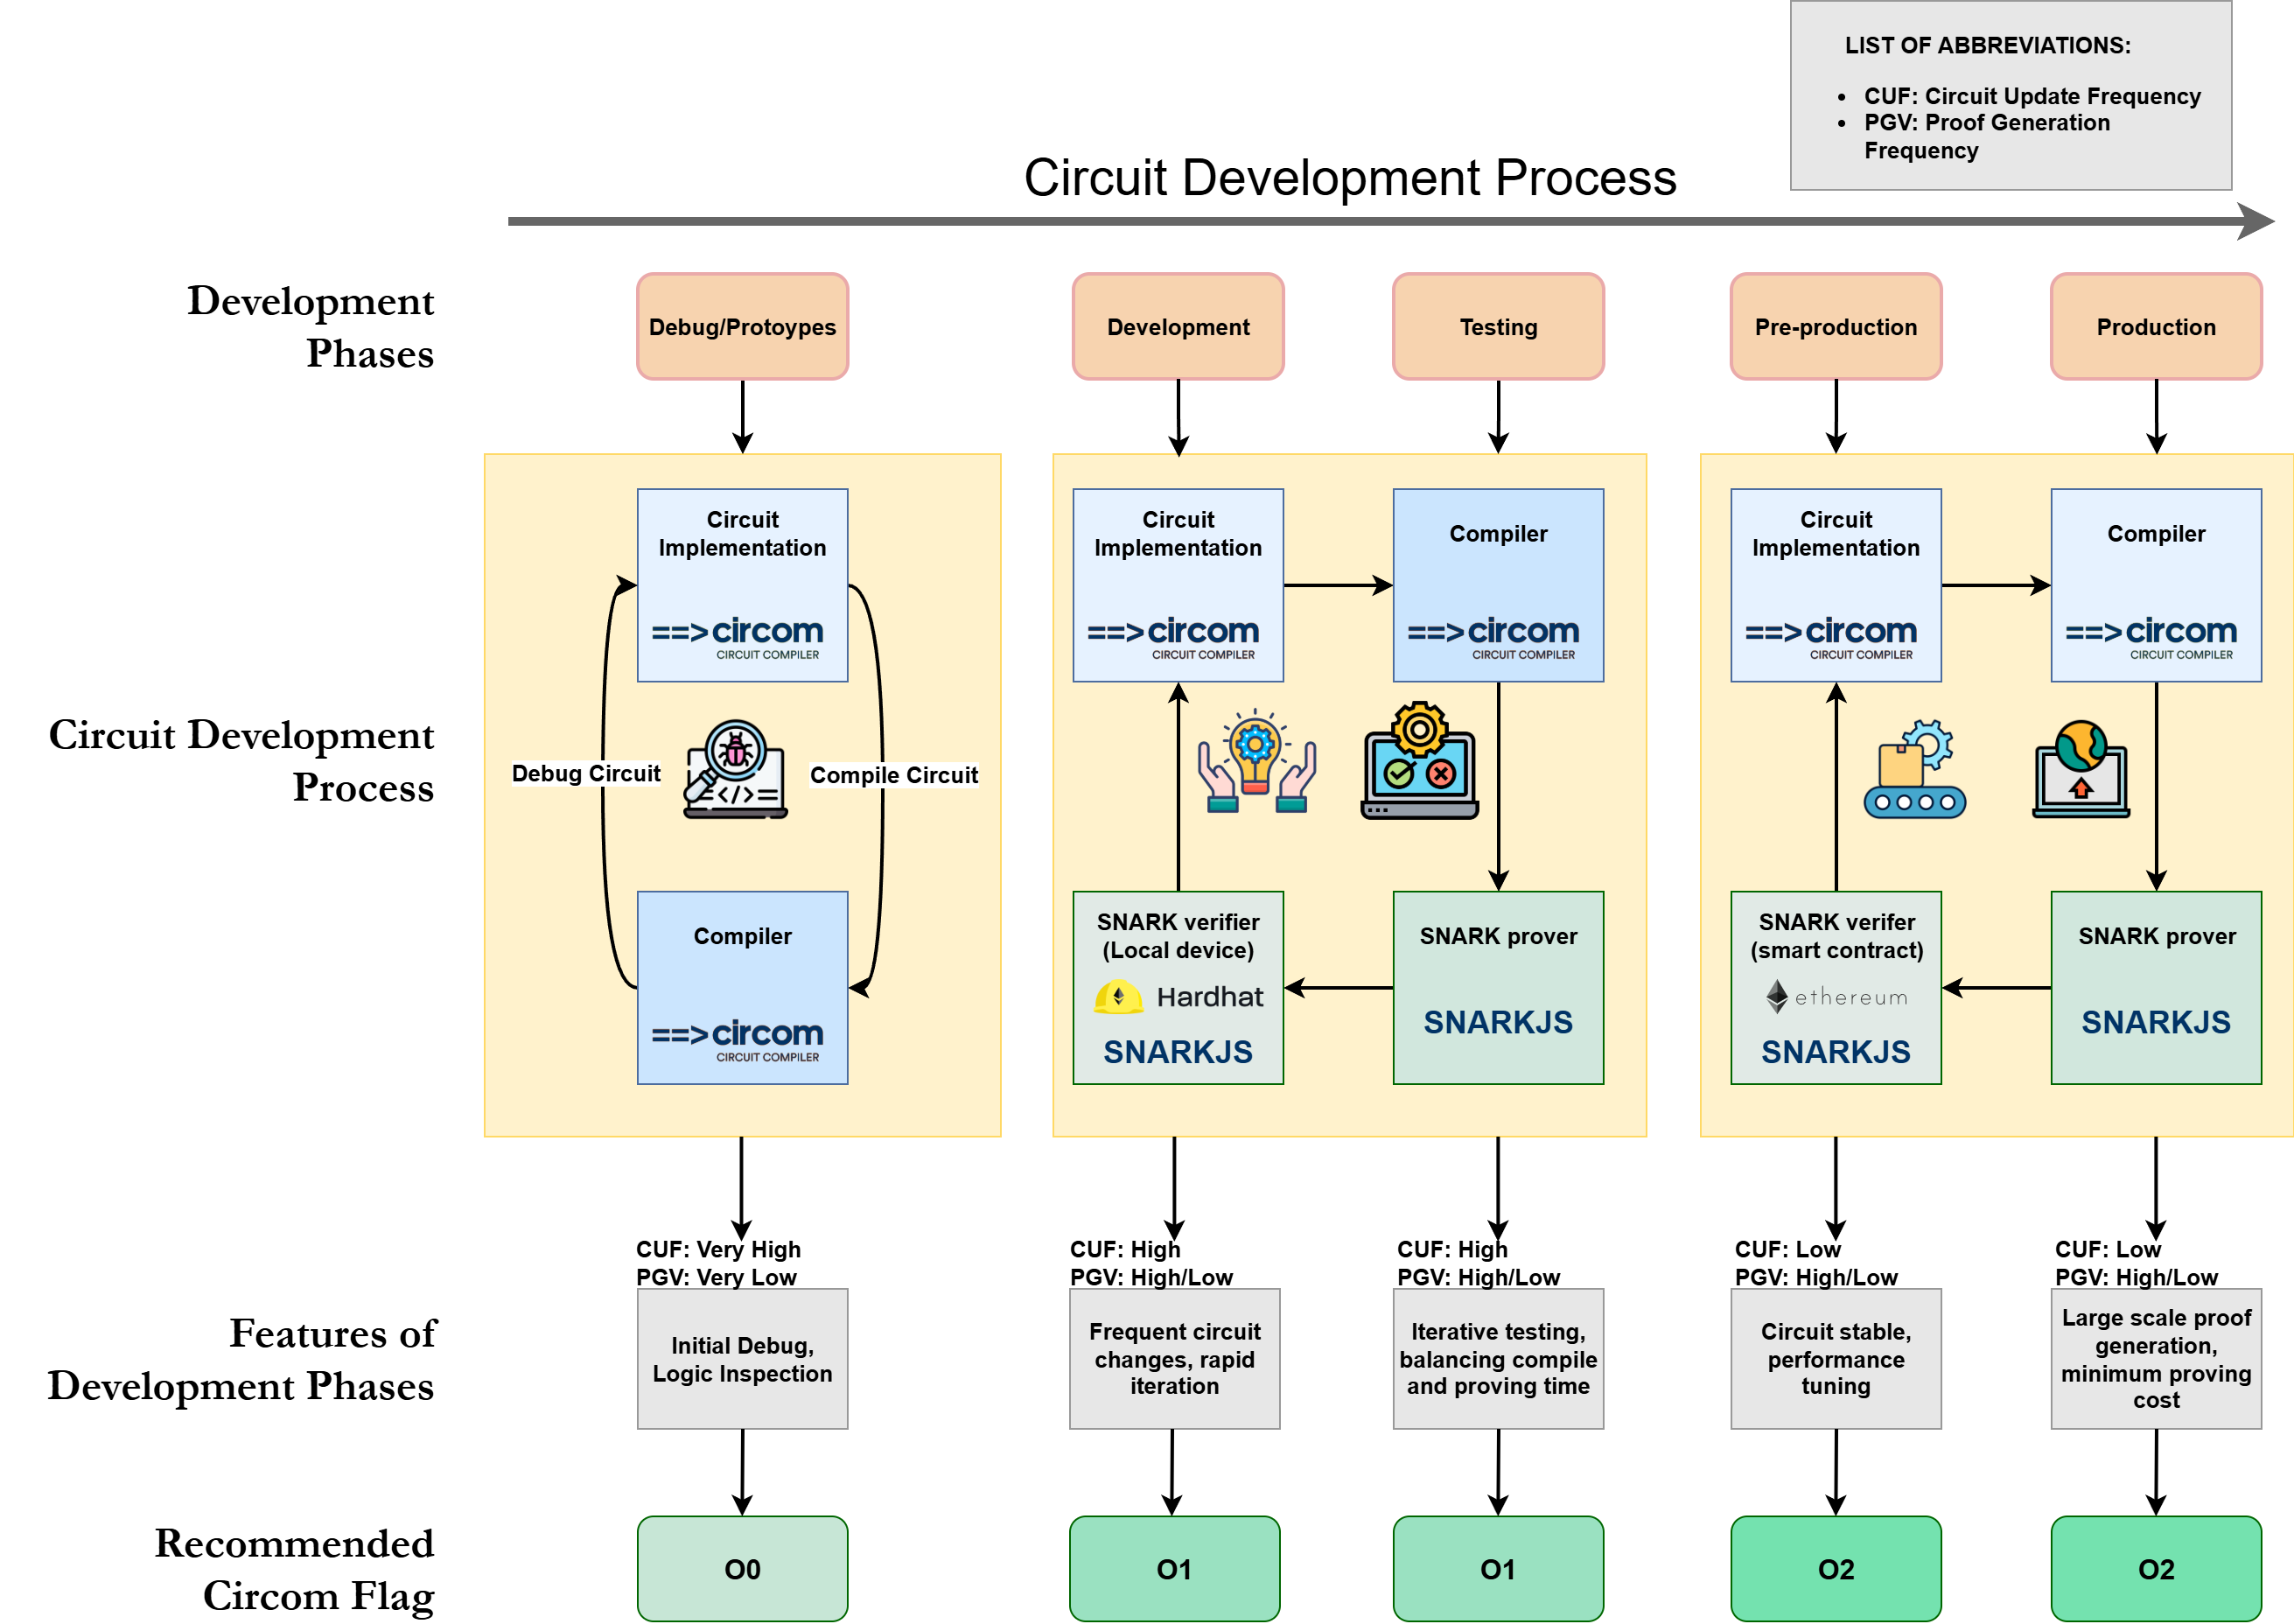
\includegraphics[height=0.9\textwidth]{imgs/FlagSelection.png}}
    \caption{Khung chọn cờ tối ưu hóa trình biên dịch Circom dựa trên giai đoạn phát triển, tần suất cập nhật mạch và khối lượng tạo bằng chứng}
    \label{fig:chapter4-FrameworkCircom}
\end{figure}
\clearpage

\section{CirMetrics: Công cụ phân tích và quản lí mạch ZKP}
\subsection{Giới thiệu}
CirMetrics là một ứng dụng hỗ trợ phát triển mạch ZKP, được em xây dựng từ nhu cầu thực tế trong việc tối ưu hóa hiệu suất biên dịch và tạo bằng chứng. Xuất phát từ nghiên cứu về chiến lược tối ưu hóa trong sử dụng trình biên dịch Circom, CirMetrics được phát triển nhằm mang lại một quy trình đánh giá hiệu quả, chính xác và trực quan hơn cho các nhà phát triển ZKP.

Ứng dụng này giúp người dùng theo dõi các thông số quan trọng trong quá trình biên dịch và tạo bằng chứng, bao gồm số lượng constraint theo từng loại, thời gian biên dịch và thời gian tạo proof. Tất cả được hiển thị bằng biểu đồ trực quan, giúp nhà phát triển dễ dàng nhận diện các vấn đề về hiệu năng và xu hướng thay đổi trong quá trình phát triển mạch.

Điểm đặc biệt của CirMetrics chính là khả năng mở rộng, hướng tới việc tích hợp các gợi ý tối ưu hóa tự động dựa trên giai đoạn phát triển của dự án. Điều này giúp các nhà phát triển Circom lựa chọn chiến lược biên dịch phù hợp, giảm chi phí tạo bằng chứng và tối ưu hóa quy trình từ nguyên mẫu đến sản phẩm hoàn chỉnh.
\subsection{Phân tích thiết kế}
Công cụ CirMetrics được thiết kế để phục vụ trực tiếp cho các nhà phát triển ứng dụng ZKP. Công cụ này được thiết kế để đáp ứng những mục tiêu như sau:

\begin{itemize}
    \item Giúp những nhà phát triển ứng dụng sử dụng ZKP có thể quản lí và theo dõi các thông số của mạch trong quá trình phát triển ứng dụng:
    \begin{itemize}
        \item Hiển thị thống kê ràng buộc: Số lượng ràng buộc tuyến tính, phi tuyến tính, tổng số ràng buộc.
        \item Theo dõi thời gian biên dịch: Đo lường thời gian biên dịch với các cờ tối ưu hóa khác nhau.
        \item Quản lí thời gian tạo bằng chứng: Người dùng có thể theo dõi và quản lí thời gian tạo bằng chứng sau mỗi lần chỉnh sửa và áp dụng các mức tối ưu ràng buộc khác nhau.
    \end{itemize}
    \item Trực quan hoá dữ liệu: Hỗ trợ hiển thị và so sánh các thông số mạch tương ứng với các mức tối ưu hóa khác nhau. Bên cạnh đó công cụ cũng hỗ trợ trực quan hoá tần suất cập nhật mạch cũng như tần suất tạo bằng chứng thông qua các biểu đồ, giúp các nhà phát triển thuận tiện hơn khi lựa chọn phương pháp tối ưu mạch trong quá trình phát triển dự án.
\end{itemize}

Bảng \ref{tab:use_case_cirmetrics} dưới đây mô tả các chức năng của CirMetrics:

\begin{table}[h]
    \centering
    \begin{tabular}{|l|p{7cm}|}
        \hline
        \textbf{Chức Năng} & \textbf{Mô Tả} \\ \hline
        Thực hiện phân tích mạch & Cho phép người viết mạch upload mạch, thực hiện biên dịch mạch và tạo bằng chứng trên giao diện công cụ CirMetrics\\ \hline
        Xem các kết quả phân tích & Hiển thị thống số của các mạch đã biên dịch và tạo bằng chứng theo thời gian. \\ \hline
        Xem tổng hợp các biểu đồ & So sánh và trực quan hóa các thông số liên quan đến mạch ZK và quá trình phát triển mạch.
        \\ \hline
    \end{tabular}
    \caption{Bảng Use Case cho công cụ CirMetrics}
    \label{tab:use_case_cirmetrics}
\end{table}
\subsection{Kiến trúc hệ thống}

CirMetrics được thiết kế theo kiến trúc Client-Server nhằm phân chia nhiệm vụ riêng biệt cho các thành phần khác nhau, giúp tối ưu hóa hiệu suất và quản lý tài nguyên tập trung. Nó cho phép mở rộng hệ thống dễ dàng và bảo vệ dữ liệu tốt hơn trên server. Kiến trúc ứng dụng này được mô tả như hình \ref{fig:chapter6-ToolsApp}, bao gồm các lớp sau:
\begin{itemize}
    \item Lớp giao diện (Front-end): Ứng dụng sử dụng ReactJS kết hợp với thư viện shadcn/ui để hỗ trợ thiết kế giao diện. Mục tiêu là giúp CirMetrics mang đến trải nghiệm trực quan và dễ sử dụng, giúp người dùng theo dõi và tương tác với dữ liệu một cách thuận tiện.
    \item Lớp xử lí nghiệp vụ (Back-end): Phần backend của CirMetrics được phát triển bằng Javascripts với NodeJS. Thành phần này chịu trách nhiệm tiếp nhận và xử lý các yêu cầu từ phía giao diện, thực hiện phân tích dữ liệu biên dịch, lưu trữ thông tin cần thiết và cung cấp API phục vụ cho giao diện.
    \item Lớp cơ sở dữ liệu (Database): Dữ liệu hệ thống được lưu trữ bằng SQLite, phù hợp với tính chất nhẹ, đơn giản và dễ triển khai cho ứng dụng hỗ trợ trong quá trình phát triển. Cơ sở dữ liệu này lưu trữ thông tin về các phiên biên dịch, số lượng constraint, thời gian thực thi và các dữ liệu phân tích liên quan.
\end{itemize}
\begin{figure}[H]
    \centering
    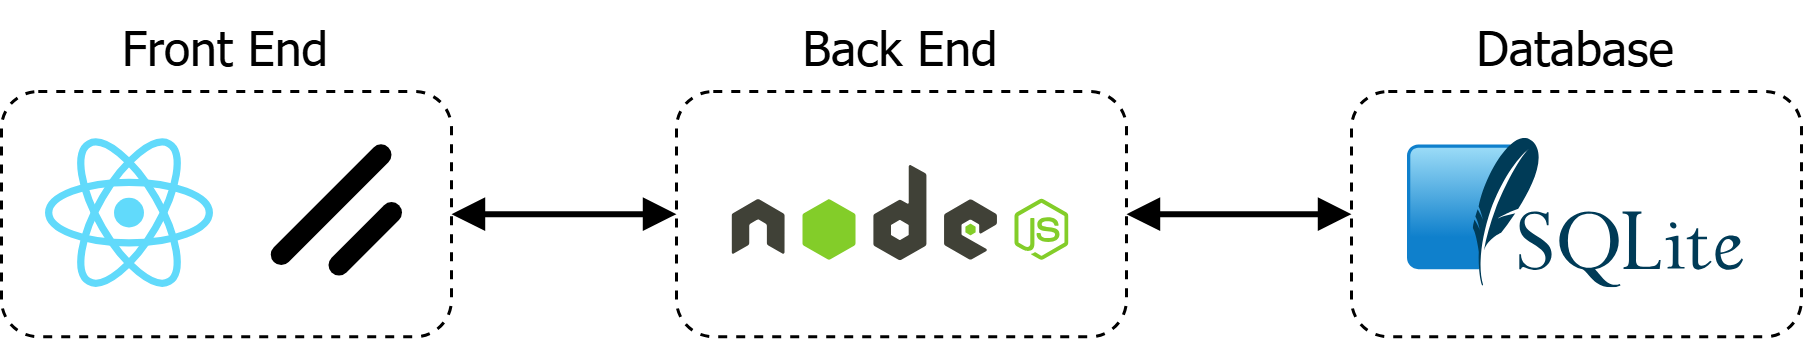
\includegraphics[width=\textwidth]{imgs/ToolsApp.png}
    \caption{Kiến trúc hệ thống CirMetrics}
    \label{fig:chapter6-ToolsApp}
\end{figure}

\subsection{CirMetrics - Demo}
Giao diện của một số tính năng của công cụ CirMetrics được trình bày dưới đây:
\subsubsection{Giao diện thực hiện phân tích mạch}
\begin{figure}[H]
    \centering
    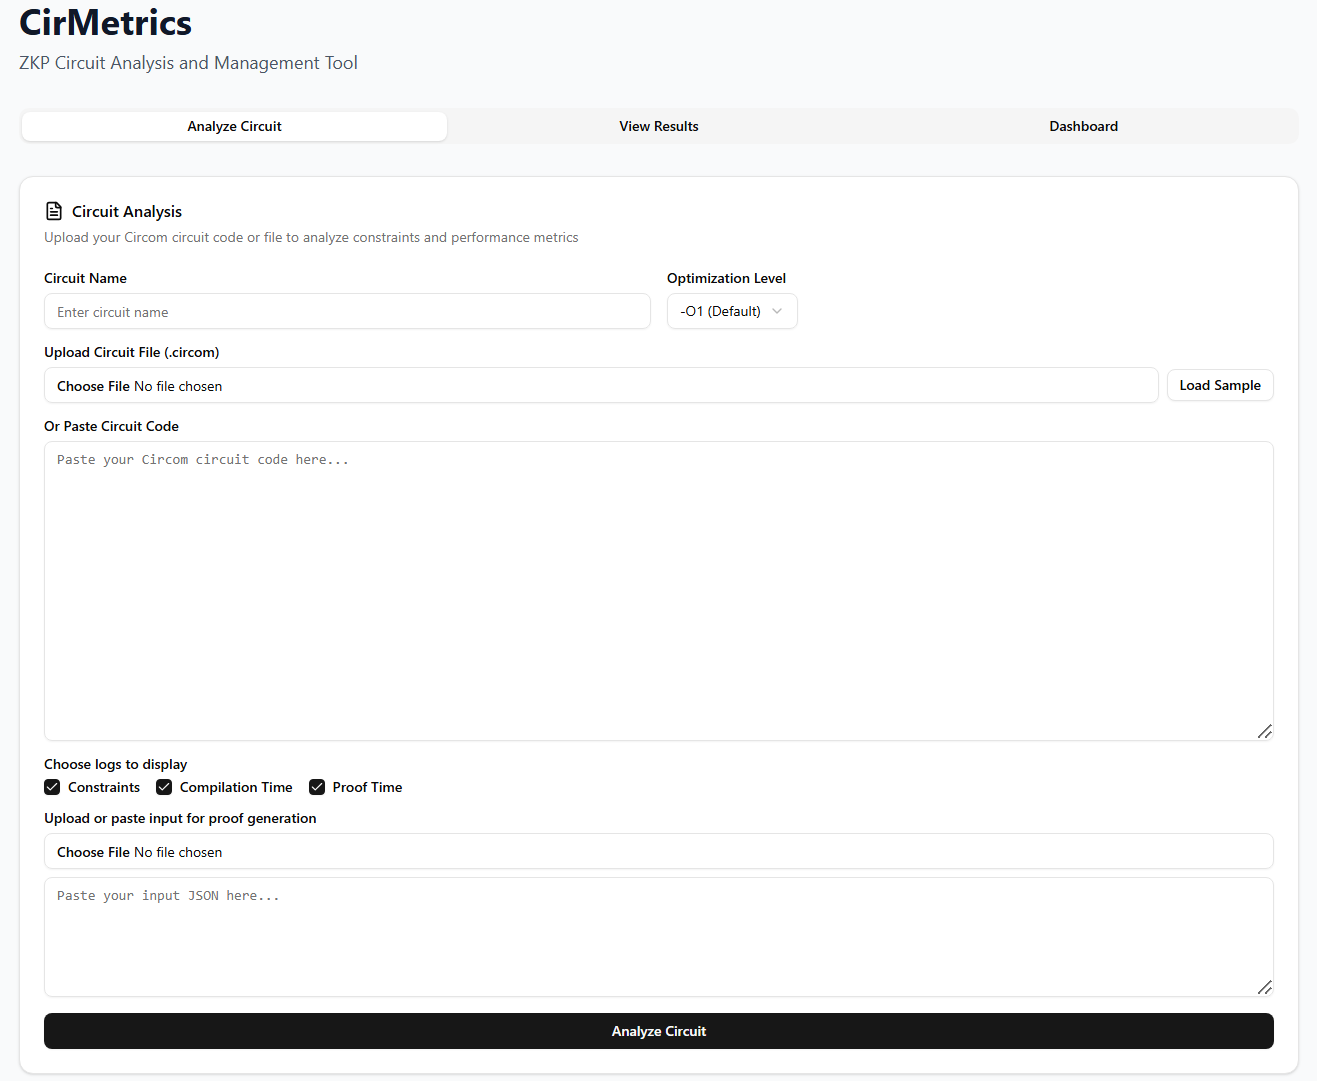
\includegraphics[width=\textwidth]{imgs/analyzescreen.png}
    \caption{Demo chức năng thực hiện phân tích mạch}
    \label{fig:chapter6-analyzescreen}
\end{figure}

Với chức năng phân tích mạch minh hoạ ở hình \ref{fig:chapter6-analyzescreen}, người dùng sẽ nhập tên mạch, sau đó upload file circom hoặc nhập mã nguồn mạch vào khung nhập liệu. Sau đó chọn các chức năng như "constraint" và "compilation time" để biên dịch và hiển thị các thống số của mạch. 

Người dùng cũng có thể chọn thêm "Proof Time" để tạo bằng chứng và nhập thêm đầu vào cho mạch ở dạng JSON để thực hiện tạo ZKP.

\subsubsection{Giao diện xem các kết quả phân tích}
\begin{figure}[H]
    \centering
    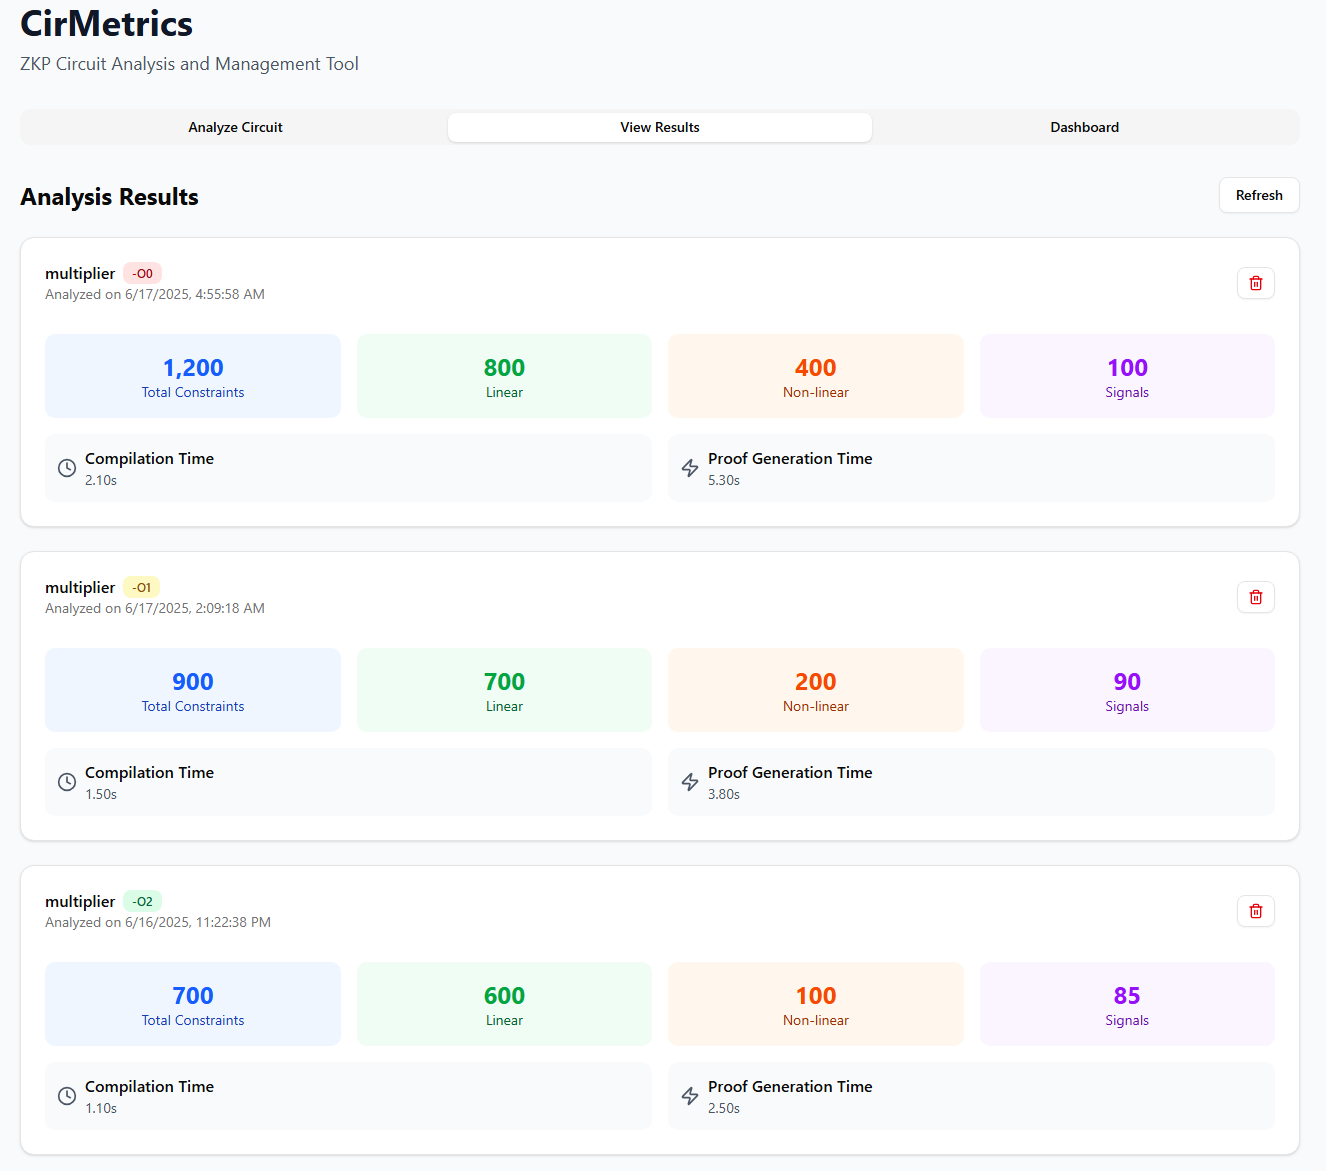
\includegraphics[width=\textwidth]{imgs/resultscreen.png}
    \caption{Demo chức năng xem các kết quả phân tích}
    \label{fig:chapter6-resultscreen}
\end{figure}

Với chức năng xem kết quả phân tích minh hoạ ở hình \ref{fig:chapter6-resultscreen}, người dung có thể xem thống số các mạch đã biên dịch và tạo bằng chứng theo thời gian. Các thông số được hiển thị bao gồm:
\begin{itemize}
    \item Thời gian biên dịch và thời gian tạo bằng chứng
    \item Số lượng ràng buộc (Tổng số lượng ràng buộc, số lượng ràng buộc tuyến tính và ràng buộc không tuyến tính).
    \item Số lượng tín hiệu của mạch.
    \item Thời gian biên dịch mạch.
    \item Thời gian tạo bằng chứng.
\end{itemize}

\subsubsection{Giao diện xem tổng hợp các biểu đồ về các thông số liên quan đến mạch ZK}

\begin{figure}[H]
    \centering
    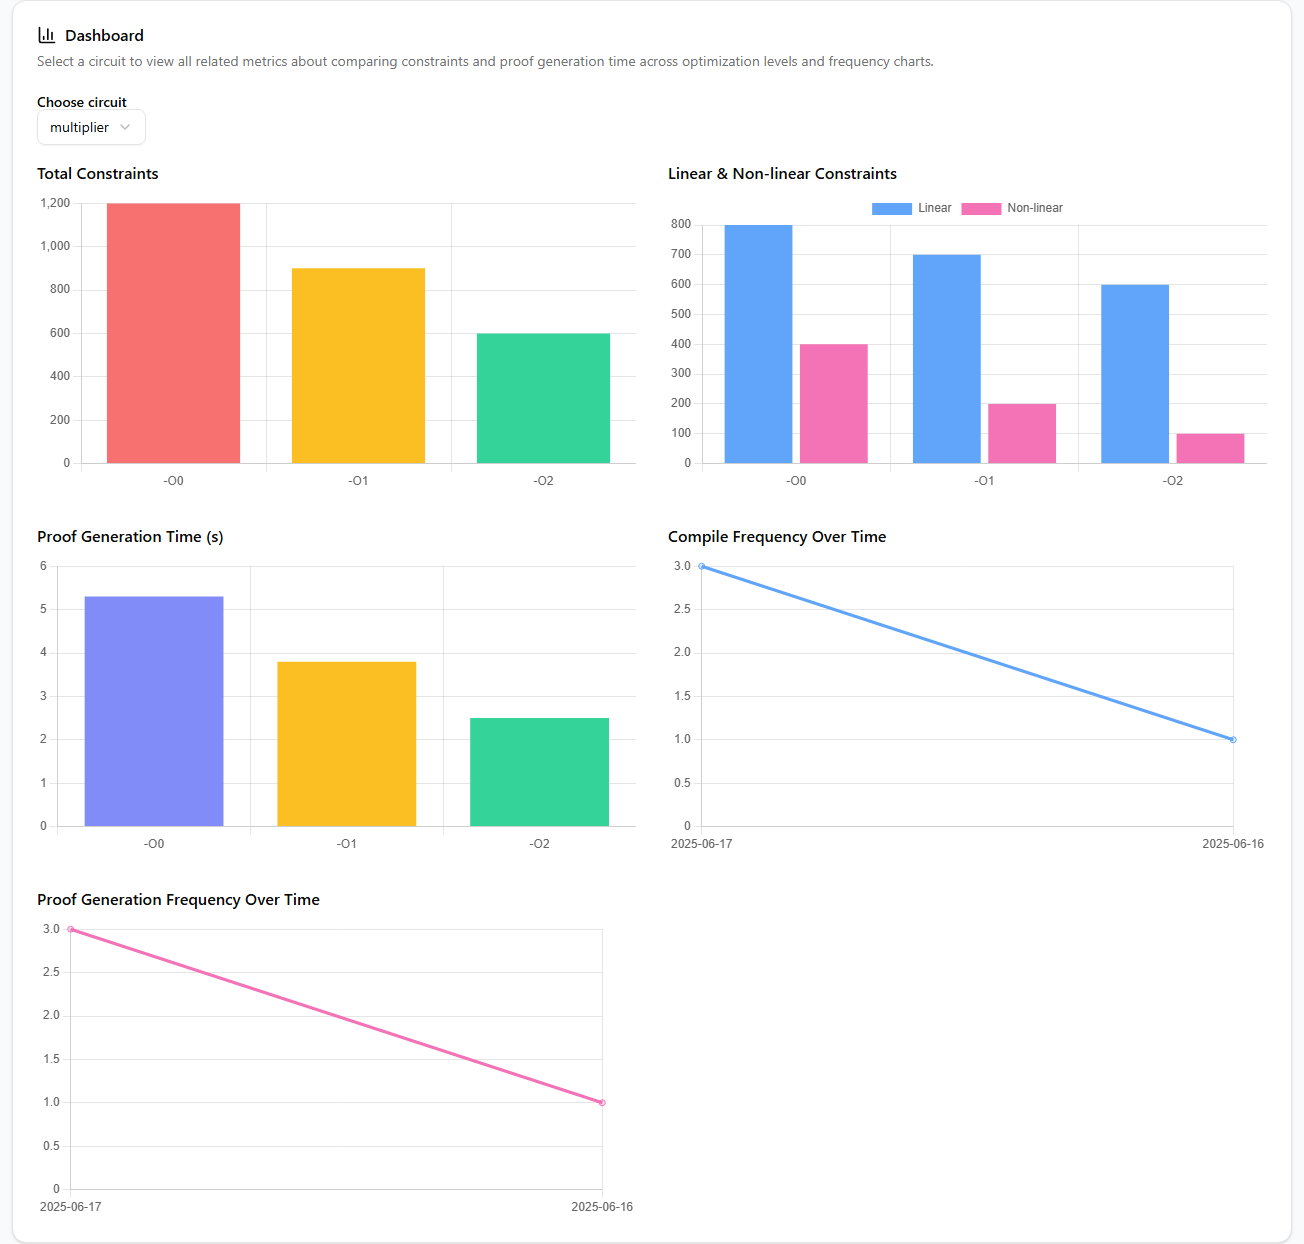
\includegraphics[width=\textwidth]{imgs/dashboardscreen.png}
    \caption{Demo chức năng xem các biểu đồ về các thông số liên quan đến mạch ZK}
    \label{fig:chapter6-dashboardscreen}
\end{figure}

Với chức năng xem các biểu đồ và thông số liên quan đến mạch ZK minh hoạ ở hình \ref{fig:chapter6-dashboardscreen}, người dùng có thể chọn tên mạch và xem các biểu đồ liên quan sau:
\begin{itemize}
    \item Biểu đồ so sánh tổng lượng constraint ở các mức tối ưu mạch khác nhau.
    \item Biểu đồ so sánh tỷ lệ giữa ràng buộc tuyến tính và ràng buộc phi tuyến.
    \item Biểu đồ so sánh thời gian tạo bằng chứng ở các mức tối ưu mạch khác nhau.
    \item Biểu đồ thể hiện tần suất cập nhật mạch và tần suất tạo bằng chứng theo ngày.
\end{itemize}

Với công cụ CirMetrics, các nhà phát triển sẽ thuận tiện hơn trong việc theo dõi trực quan các thông số khi làm việc với mạch ZK. Đồng thời hỗ trợ các nhà phát triển trong việc đưa ra những quyết định hợp lí hơn khi kết hợp công cụ cùng khung \textbf{ZCLS} khi chọn phương án tối ưu hoá mạch phù hợp cho tiến trình phát triển mạch của mình.